\newpage
\section{PHƯƠNG TRÌNH ĐƯỜNG THẲNG TRONG KHÔNG GIAN}
\subsection{LÝ THUYẾT CẦN NHỚ}
\subsubsection{Phương trình đường thẳng trong không gian}
\indam{Vectơ chỉ phương của đường thẳng}
	\begin{boxdn}
		Vectơ $\overrightarrow{a}$ khác $\overrightarrow{0}$ có giá song song hoặc trùng với đường thẳng $d$ được gọi là \textbf{\textit{vectơ chỉ phương}} của $d$.
		\begin{center}
			\begin{tikzpicture}[scale=1, font=\footnotesize, line join=round, line cap=round, >=stealth]
			\draw[blue] (0,0)--(3,2) node[above] {$d$};
			\draw[red, ->] (0.5,1)--($(0.5,1)+(1.5,1)$) node[midway, above] {$\overrightarrow{a}$};
		\end{tikzpicture}
		\end{center}
	\end{boxdn}
	
\begin{khung4}{Chú ý}
	Nếu $\overrightarrow{a}$ là véc-tơ chỉ phương của $d$ thì $k\overrightarrow{a}$ ($k\neq 0$) cũng là véc-tơ chỉ phương của $d$.
\end{khung4}

\indam{Phương trình tham số của đường thẳng}
\begin{boxdn}
	Trong không gian $Oxyz$, \textbf{\textit{phương trình tham số}} của đường thẳng $d$ đi qua $M_0(x_0;y_0;z_0)$ và nhận $\overrightarrow{a}=(a_1;a_2;a_3)$ làm véc-tơ chỉ phương có dạng
	$$\heva{&x=x_0+a_1t\\&y=y_0+a_2t\\&z=z_0+a_3t} \text{ với }t\in \mathbb{R} \text{ ($t$ được gọi là tham số)}.  $$
\end{boxdn}

\begin{khung4}{Chú ý}
	\begin{enumerate}
		\item Trong phương trình tham số của đường thẳng $d\colon \heva{&x=x_0+a_1t\\&y=y_0+a_2t\\&z=z_0+a_3t}$, mỗi giá trị của tham số $t$ xác định duy nhất một điểm $M$ trên $d$ và ngược lại.
		\item Từ nay để cho gọn, trong phương trình tham số của đường thẳng, ta không viết $t\in \mathbb{R}$.
	\end{enumerate}
\end{khung4}

\indam{Phương trình chính tắc của đường thẳng}
\begin{boxdn}
	Trong không gian $Oxyz$, cho đường thẳng $d$ đi qua $M(x_0;y_0;z_0)$ và có véc-tơ chỉ phương $\overrightarrow{a}=(a_1;a_2;a_3)$.\\ 
	Nếu $a_1$, $a_2$, $a_3$ đều khác $0$ thì hệ phương trình
	$$\dfrac{x-x_0}{a_1}=\dfrac{y-y_0}{a_2}=\dfrac{z-z_0}{a_3}.$$
	gọi là \textbf{\textit{phương trình chính tắc}} của đường thẳng $d$.
\end{boxdn}

\indam{Viết phương trình tham số, phương trình chính tắc của đường thẳng đi qua hai điểm}
\begin{boxdn}
	Trong không gian $Oxyz$, cho đường thẳng $d$ đi qua hai điểm phân biệt $A(x_A;y_A;z_A)$, $B(x_B;y_B;z_B)$ có véc-tơ chỉ phương là $\overrightarrow{AB}=(x_B-x_A;y_B-y_A;z_B-z_A)$ và có phương trình tham số
	$$\heva{&x=x_A+(x_B-x_A)t\\&y=y_A+(y_B-y_A)t\\&z=z_A+(z_B-z_A)t.} $$
	Nếu $x_A\neq x_B$, $y_A\neq y_B$, $z_A\neq z_B$ thì $d$ có phương trình chính tắc
	$$\dfrac{x-x_A}{x_B-x_A}=\dfrac{y-y_A}{y_B-y_A}=\dfrac{z-z_A}{z_B-z_A}$$
\end{boxdn}

\subsubsection{Vị trí tương đối giữa hai đường thẳng. Điều kiện để hai đường thẳng vuông góc}
\indam{Điều kiện để hai đường thẳng song song hoặc trùng nhau}
\begin{boxdn}
	Gọi $\overrightarrow{a}=(a_1;a_2;a_3)$ và $\overrightarrow{a'}=(a'_1;a'_2;a'_3)$ lần lượt là véc-tơ chỉ phương của hai đường thẳng $d$ và $d'$. Gọi $M(x_0;y_o;z_0)$ là một điểm trên $d$. Ta có
	\begin{multicols}{2}
		\begin{enumerate}
			\item $d \parallel d'\Leftrightarrow \heva{&\overrightarrow{a}=k\overrightarrow{a'}\quad (k\in \mathbb{R})\\&M\notin d'}$.
			\item $d\equiv d'\Leftrightarrow \heva{&\overrightarrow{a}=k\overrightarrow{a'}\quad (k\in \mathbb{R})\\&M\in d'}$.
		\end{enumerate}
	\end{multicols}
	\begin{center}
		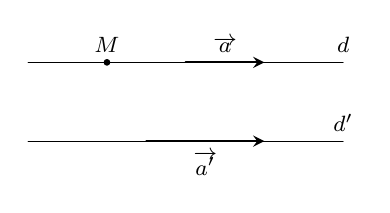
\begin{tikzpicture}[scale=1, font=\footnotesize, line join=round, line cap=round, >=stealth]
			\draw (0,0)--(4,0) node[above] {$d$};
			\draw (0,-1)--(4,-1) node[above] {$d'$};
			\draw[fill=black] (1,0) circle (1pt) node[above] {$M$};
			\draw[thick, ->] (2,0)--(3,0) node[midway, above] {$\overrightarrow{a}$};
			\draw[thick, ->] (1.5,-1)--(3,-1) node[midway, below] {$\overrightarrow{a'}$};
		\end{tikzpicture}
	\end{center}
\end{boxdn}

\begin{khung4}{Chú ý}
	Cho đường thẳng $d$ đi qua điểm $M$ và có véc-tơ chỉ phương $\overrightarrow{a}$, đường thẳng $d'$ đi qua điểm $M'$ và có véc-tơ chỉ phương $\overrightarrow{a'}$.
	\begin{enumerate}
		\item Nếu ba véc-tơ $\overrightarrow{a}$, $\overrightarrow{a'}$, $\overrightarrow{MM'}$ cùng phương thì $d\equiv d'$.
		\item Nếu hai véc-tơ $\overrightarrow{a}$, $\overrightarrow{a'}$ cùng phương và hai véc-tơ  $\overrightarrow{a}$, $\overrightarrow{MM'}$ không cùng phương thì $d\parallel d'$.
	\end{enumerate}
\end{khung4}

\indam{Điều kiện để hai đường thẳng cắt nhau hoặc chéo nhau}
\begin{boxdn}
	Xét hệ phương trình ẩn $t$ và $t'$ $\heva{&x_0+a_1t=x'_0+a'_1t'\\&y_0+a_2t=y'_0+a'_2t'\\&z_0+a_3t=z'_0+a'_3t'}$
	\begin{enumerate}
		\item $d$ và $d'$ cắt nhau khi và chỉ khi hệ trên có đúng một nghiệm.
		\item $d$ và $d'$ chéo nhau khi và chỉ khi $\overrightarrow{a}$, $\overrightarrow{a'}$ không cùng phương và hệ trên vô nghiệm.
	\end{enumerate}
	\begin{center}
		\begin{tikzpicture}[scale=1, font=\footnotesize, line join=round, line cap=round, >=stealth]
			\draw (0,0)--(4,2) node[above] {$d$};
			\draw (0,-1)--(4,-2) node[above] {$d'$};
			\draw[thick, ->] ($(0,0)!0.3!(4,2)$)--($(0,0)!0.6!(4,2)$) node[midway, above] {$\overrightarrow{a}$};
			\draw[thick, ->] ($(0,-1)!0.3!(4,-2)$)--($(0,-1)!0.6!(4,-2)$) node[midway, below] {$\overrightarrow{a'}$};
		\end{tikzpicture}
	\end{center}
\end{boxdn}

\begin{khung4}{Chú ý $1$}
	Để xét vị trí tương đối của $d$ và $d'$, trước hết ta kiểm tra tính cùng phương của hai véc-tơ chỉ phương của $d$ và $d'$.
	\begin{enumerate}
		\item Nếu $\overrightarrow{a}$ và $\overrightarrow{a'}$ cùng phương thì $d$ và $d'$ hoặc song song hoặc trùng nhau.
		\item Nếu $\overrightarrow{a}$ và $\overrightarrow{a'}$ không cùng phương thì $d$ và $d'$ hoặc cắt nhau hoặc chéo nhau.
	\end{enumerate}
\end{khung4}

\begin{khung4}{Chú ý $2$}
	Cho đường thẳng $d$ đi qua điểm $M$ và có véc-tơ chỉ phương $\overrightarrow{a}$, đường thẳng $d'$ đi qua điểm $M'$ và có véc-tơ chỉ phương $\overrightarrow{a'}$.\\ 
	Trong trường hợp $\overrightarrow{a}$, $\overrightarrow{a'}$ không cùng phương, nghĩa là $\left[\overrightarrow{a},\overrightarrow{a'}\right]\neq \overrightarrow{0}$, ta có
	\begin{itemize}
		\item Nếu $\left[\overrightarrow{a},\overrightarrow{a'}\right]\cdot \overrightarrow{MM'}=0$ thì $d$ và $d'$ cắt nhau.
		\item Nếu $\left[\overrightarrow{a},\overrightarrow{a'}\right]\cdot \overrightarrow{MM'}\neq 0$ thì $d$ và $d'$ chéo nhau.
	\end{itemize}
\end{khung4}

\indam{Điều kiện để hai đường thẳng vuông góc}
\begin{boxdn}
	Cho hai đường thẳng $d$ và $d'$ có véc-tơ chỉ phương lần lượt là $\overrightarrow{a}=(a_1;a_2;a_3)$ và $\overrightarrow{a'}=(a'_1;a'_2;a'_3)$. Ta có
	$$d\perp d' \Leftrightarrow \overrightarrow{a}\cdot \overrightarrow{a'}=0\Leftrightarrow a_1a'_1+a_2a'_2+a_3a'_3=0.$$
\end{boxdn}

\subsubsection{Góc}

\indam{Góc giữa hai đường thẳng}
\begin{boxdn}
	Góc giữa hai đường thẳng $d$ và $d'$ có véc-tơ chỉ phương lần lượt là $\overrightarrow{a}=(a_1;a_2;a_3)$ và $\overrightarrow{a'}=(a'_1;a'_2;a'_3)$ được tính bởi công thức
	$$
		\cos(d,d')=\left|\cos(\overrightarrow{a},\overrightarrow{a'})\right|=\dfrac{\left|\overrightarrow{a}\cdot \overrightarrow{a'}\right|}{\left|\overrightarrow{a}\right|\cdot \left|\overrightarrow{a'}\right|} 
		=\dfrac{\left|a_1a'_1+a_2a'_2+a_3a'_3\right|}{\sqrt{{a_1}^2+{a_2}^2+{a_3}^2}\cdot \sqrt{{a'_1}^2+{a'_2}^2+{a'_3}^2}}.
	$$
\end{boxdn}

\indam{Góc giữa đường thẳng và mặt phẳng}
\begin{boxdn}
	Góc giữa đường thẳng $d$ có véc-tơ chỉ phương $\overrightarrow{a}=(a_1;a_2;a_3)$ và mặt phẳng $(P)$ có véc-tơ pháp tuyến $\overrightarrow{n}=(n_1;n_2;n_3)$ được tính bởi công thức
	$$
		\sin(d,(P))=\left|\cos(\overrightarrow{a},\overrightarrow{n})\right|=\dfrac{\left|\overrightarrow{a}\cdot \overrightarrow{n}\right|}{\left|\overrightarrow{a}\right|\cdot \left|\overrightarrow{n}\right|} 
		= \dfrac{\left|a_1n_1+a_2n_2+a_3n_3\right|}{\sqrt{{a_1}^2+{a_2}^2+{a_3}^2}\cdot \sqrt{{n_1}^2+{n_2}^2+{n_3}^2}}.
	$$
\end{boxdn}

\begin{khung4}{Chú ý}
	Nếu đường thẳng $d$ có véc-tơ chỉ phương cùng phương với pháp tuyến của mặt phẳng $(P)$ thì $d$ vuông góc với $(P)$.
\end{khung4}

\indam{Góc giữa hai mặt phẳng}
\begin{boxdn}
	Góc giữa hai mặt phẳng $(P)$ và $(P')$ có véc-tơ pháp tuyến lần lượt là $\overrightarrow{n}=(n_1;n_2;n_3)$ và $\overrightarrow{n'}=(n'_1;n'_2;n'_3)$ được tính bởi công thức
	$$
		\cos((P),(P'))=\left|\cos(\overrightarrow{n},\overrightarrow{n'})\right|=\dfrac{\left|\overrightarrow{n}\cdot \overrightarrow{n'}\right|}{\left|\overrightarrow{n}\right|\cdot \left|\overrightarrow{n'}\right|} 
		=\dfrac{\left|n_1n'_1+n_2n'_2+n_3n'_3\right|}{\sqrt{{n_1}^2+{n_2}^2+{n_3}^2}\cdot \sqrt{{n'_1}^2+{n'_2}^2+{n'_3}^2}}.
	$$
\end{boxdn}
%-------------------------------------------------------------------------------------------------------------
\subsection{PHÂN LOẠI VÀ PHƯƠNG PHÁP GIẢI TOÁN}
\begin{dang}{Xác định các yếu tố cơ bản của đường thẳng trong không gian. Vị trí tương đối trong không gian}
	Trong không gian $Oxyz$, véc-tơ $\overrightarrow{a}=(a_1;a_2;a_3)$ là véc-tơ chỉ phương của đường thẳng $d$ thì véc-tơ $\overrightarrow{a'}=k\overrightarrow{a}$ cũng là véc-tơ chỉ phương của đường thẳng $d$.\\ 
	Phương trình tham số $d\colon \heva{&x=x_0+a_1t\\&y=y_0+a_2t\\&z=z_0+a_3t}$ có véc-tơ chỉ phương $\overrightarrow{a}=(a_1;a_2;a_3)$ (hệ số trước $t$).\\ 
	Phương trình chính tắc $d\colon \dfrac{x-x_0}{a_1}=\dfrac{y-y_0}{a_2}=\dfrac{z-z_0}{a_3}$ có véc-tơ chỉ phương $\overrightarrow{a}=(a_1;a_2;a_3)$ (hệ số ở mẫu).\\ 
	\textbf{Nhận xét}
	\begin{itemize}
		\item Với phương trình tham số lấy đúng thứ tự hệ số trước tham số $t$.
		\item Với phương trình chính tắc lấy hệ số dưới mẫu.
		\item Nếu giả thiết chưa đúng cấu trúc, ta phải sắp xếp lại rồi mới lấy hệ số.
	\end{itemize}
\end{dang}

\begin{vd}%[2H5N2-2]%[Dự án đề cương 3 Khối NH24-25-Dot 1-Viet Hoang Pham]
	Trong không gian $Oxyz$, xác định một véc-tơ chỉ phương của đường thẳng dưới đây:
	\begin{multicols}{3}
		\begin{enumerate}
			\item[a)] $d\colon\heva{&x=2-t\\&y=1+2t\\&z=3+t}$
			\item[b)] $d\colon\dfrac{x-1}{2}=\dfrac{y-2}{1}=\dfrac{z+1}{2}$
			\item[c)] $d\colon\dfrac{x-1}{2}=\dfrac{y-1}{2}=\dfrac{2-z}{1}$
		\end{enumerate}
	\end{multicols}
	\loigiai{
		\begin{enumerate}
			\item[a)] Đường thẳng $d$ có một véc-tơ chỉ phương là $\overrightarrow{u}=(-1;2;1)$.
			\item[b)] Đường thẳng $d$ có một véc-tơ chỉ phương là $\overrightarrow{v}=(2;1;2)$.
			\item[c)] Ta viết lại $d\colon\dfrac{x-1}{2}=\dfrac{y-1}{2}=\dfrac{z-2}{-1}$.\\
			Suy ra, đường thẳng $d$ có một véc-tơ chỉ phương là $\overrightarrow{w}=(2;2;-1)$.
		\end{enumerate}
	}
\end{vd}
\begin{vd}%[2H2N2-2]%[Dự án đề cương 3 Khối NH24-25-Dot 1-Viet Hoang Pham]
	\immini{Cho hình hộp $ABCD.A'B'C'D'$. Trong các véc-tơ có điểm đầu và điểm cuối là các đỉnh của hình hộp, những véc-tơ nào là véc-tơ chỉ phương của đường thẳng $AC$?}
	{
		\begin{tikzpicture}[scale=1, font=\footnotesize, line join=round, line cap=round, >=stealth]
			\coordinate (A) at (0,0);
			\coordinate (B) at (-1.5,-0.5);
			\coordinate (D) at (2,0);
			\coordinate (C) at ($(B)+(D)-(A)$);
			\coordinate (A') at (0.5,2);
			\coordinate (B') at ($(B)+(A')-(A)$);
			\coordinate (C') at ($(C)+(A')-(A)$);
			\coordinate (D') at ($(D)+(A')-(A)$);
			
			\draw (B)--(C)--(D);
			\draw (B)--(B')--(A')--(D')--(C')--(B');
			\draw (C)--(C');
			\draw (D)--(D');
			\draw[dashed] (A)--(B);
			\draw[dashed] (A)--(D);
			\draw[dashed] (A)--(A');
			
			\node[below left] at (A) {$A$};
			\node[below left] at (B) {$B$};
			\node[below right] at (C) {$C$};
			\node[below right] at (D) {$D$};
			\node[above left] at (A') {$A'$};
			\node[above left] at (B') {$B'$};
			\node[above right] at (C') {$C'$};
			\node[above right] at (D') {$D'$};
		\end{tikzpicture}
	}
	\loigiai{
		Vì $AC$ song song với $A'C'$ nên các véc-tơ chỉ phương của đường thẳng $AC$ thỏa bài toán là các véc-tơ sau đây: $\overrightarrow{AC}, \overrightarrow{CA}, \overrightarrow{A'C'}, \overrightarrow{C'A'}$.
	}
\end{vd}
\begin{vd}%[2H5H2-4]%[Dự án đề cương 3 Khối NH24-25-Dot 1-Viet Hoang Pham]
	Trong không gian $Oxyz$, xét vị trí tương đối của các cặp đường thẳng sau:
	\begin{enumerate}
		\item[a)] $d\colon\heva{&x=1+t\\&y=2t\\&z=3-t}$ ($t\in\mathbb{R}$) và $d'\colon\heva{&x=2+2t'\\&y=4t'\\&z=5-2t'}$ ($t'\in\mathbb{R}$)
		\item[b)] $d\colon\heva{&x=1+2t\\&y=-1+3t\\&z=5+t}$ ($t\in\mathbb{R}$) và $d'\colon\dfrac{x-1}{3}=\dfrac{y+2}{2}=\dfrac{z+1}{2}$
		\item[c)] $d\colon\dfrac{x}{1}=\dfrac{y-1}{-1}=\dfrac{z}{2}$ và $d'\colon\dfrac{x-1}{5}=\dfrac{y-2}{-1}=\dfrac{z+2}{-2}$
	\end{enumerate}
	\loigiai{
		\begin{enumerate}
			\item[a)] Đường thẳng $d$ có VTCP $\overrightarrow{u}_1=(1;2;-1)$.\\
			Đường thẳng $d'$ có VTCP $\overrightarrow{u}_2=(2;4;-2)$.\\
			Ta có $\overrightarrow{u}_2=2\overrightarrow{u}_1$ nên hai véc-tơ này cùng phương, suy ra $d$ song song hoặc trùng với $d'$.\\
			Lấy điểm $M(1;0;3)$ thuộc $d$ (ứng với $t=0$). Thay vào phương trình của $d'$:
			$\heva{&1=2+2t'\\&0=4t'\\&3=5-2t'}\Leftrightarrow\heva{&t'=-1/2\\&t'=0\\&t'=1}$. Hệ vô nghiệm.\\
			Vậy $M\notin d'$, do đó hai đường thẳng $d$ và $d'$ song song.

			\item[b)] Đường thẳng $d$ có VTCP $\overrightarrow{u}_1=(2;3;1)$.\\
			Đường thẳng $d'$ có VTCP $\overrightarrow{u}_2=(3;2;2)$.\\
			Vì $\overrightarrow{u}_1$ và $\overrightarrow{u}_2$ không cùng phương nên $d$ và $d'$ cắt nhau hoặc chéo nhau.\\
			Xét hệ phương trình giao điểm: $\heva{&1+2t=1+3t'\\&-1+3t=-2+2t'\\&5+t=-1+2t'}$ ($I$).\\
			Từ hai phương trình đầu ta có hệ: $\heva{&2t-3t'=0\\&3t-2t'=-1}\Leftrightarrow\heva{&t=-3/5\\&t'=-2/5}$.\\
			Thay vào phương trình thứ ba: $5+\left(-\dfrac{3}{5}\right) = -1+2\left(-\dfrac{2}{5}\right) \Leftrightarrow \dfrac{22}{5} = -\dfrac{9}{5}$ (vô lý).\\
			Hệ ($I$) vô nghiệm. Vậy hai đường thẳng $d$ và $d'$ chéo nhau.

			\item[c)] Đường thẳng $d$ có VTCP $\overrightarrow{u}_1=(1;-1;2)$.\\
			Đường thẳng $d'$ có VTCP $\overrightarrow{u}_2=(5;1;-2)$.\\
			Vì $\overrightarrow{u}_1$ và $\overrightarrow{u}_2$ không cùng phương nên $d$ và $d'$ cắt nhau hoặc chéo nhau.\\
			Phương trình tham số của $d$ là $\heva{&x=t\\&y=1-t\\&z=2t}$. Phương trình tham số của $d'$ là $\heva{&x=1+5t'\\&y=2+t'\\&z=-2-2t'}$.\\
			Xét hệ phương trình giao điểm: $\heva{&t=1+5t'\\&1-t=2+t'\\&2t=-2-2t'}\Leftrightarrow\heva{&t=-\dfrac{2}{3}\\&t'=-\dfrac{1}{3}}$.\\
			Hệ có nghiệm duy nhất. Vậy hai đường thẳng $d$ và $d'$ cắt nhau.
		\end{enumerate}
	}
\end{vd}

\begin{dang}{Viết phương trình đường thẳng}
	Ta thường gặp các dạng toán sau:
	\begin{enumerate}
		\item Đường thẳng đi qua một điểm $M(x_0;y_0;z_0)$ và có một vecto chỉ phương $\overrightarrow{a}=(a_1;a_2;a_3)$.\\ 
		Khi đó phương trình đường thẳng là\\ 
		$\heva{&x=x_0+a_1t\\&y=y_0+a_2t\\&z=z_0+a_3t}$ hoặc $\dfrac{x-x_0}{a_1}=\dfrac{y-y_0}{a_2}=\dfrac{z-z_0}{a_3}$ nếu $a$, $b$, $c\neq 0$.\\ 
		\item Phương trình đường thẳng đi qua hai điểm $A(a_1;a_2;a_3)$ và $B(b_1;b_2;b_3)$\\ 
		Chọn $A$ hoặc $B$ là điểm mà đường thẳng đi qua, vecto chỉ phương là $\overrightarrow{a}=\overrightarrow{AB}=(b_1-a_1;b_2-a_2;b_3-a_3)$.\\ 
		Nếu phương trình tìm được không nằm trong các phương án, ta có thể thay tọa độ điểm mà đường thẳng đi qua để kiểm tra.
	\end{enumerate}
\end{dang}
\setcounter{vd}{0}
%Ví dụ 1
\begin{vd}%[2H5H2-3]%[Dự án đề cương 3 Khối NH24-25-Dot 1-Viet Hoang Pham]
	Trong không gian $Oxyz$, viết các phương trình tham số và chính tắc của đường thẳng $\Delta$ đi qua $A(1;1;2)$ và song song với đường thẳng $d\colon\dfrac{x-3}{2}=\dfrac{y-1}{1}=\dfrac{z+5}{3}$.
	\loigiai{
		Đường thẳng $d$ có véc-tơ chỉ phương là $\overrightarrow{u}=(2;1;3)$.\\
		Vì $\Delta \parallel d$ nên véc-tơ chỉ phương của $\Delta$ là $\overrightarrow{u}_{\Delta}=(2;1;3)$.\\
		Đường thẳng $\Delta$ đi qua điểm $A(1;1;2)$ và có véc-tơ chỉ phương là $\overrightarrow{u}_{\Delta}=(2;1;3)$.\\
		Phương trình tham số của $\Delta$ là $\heva{&x=1+2t\\&y=1+t\\&z=2+3t}$ ($t\in\mathbb{R}$).\\
		Phương trình chính tắc của $\Delta$ là $\dfrac{x-1}{2}=\dfrac{y-1}{1}=\dfrac{z-2}{3}$.
	}
\end{vd}
\begin{vd}%[2H5H2-3]%[Dự án đề cương 3 Khối NH24-25-Dot 1-Viet Hoang Pham]
	Trong không gian $Oxyz$, viết các phương trình tham số và chính tắc của đường thẳng $\Delta$ đi qua $A(2;-1;4)$ và vuông góc với mặt phẳng $(P)\colon x+3y-z-1=0$.
	\loigiai{
		Mặt phẳng $(P)$ có véc-tơ pháp tuyến là $\overrightarrow{n}=(1;3;-1)$.\\
		Vì $\Delta\perp (P)$ nên véc-tơ chỉ phương của $\Delta$ là $\overrightarrow{u}=\overrightarrow{n}=(1;3;-1)$.\\
		Đường thẳng $\Delta$ đi qua điểm $A(2;-1;4)$ và có véc-tơ chỉ phương là $\overrightarrow{u}=(1;3;-1)$.\\
		Phương trình tham số của $\Delta$ là $\heva{&x=2+t\\&y=-1+3t\\&z=4-t}$ ($t\in\mathbb{R}$).\\
		Phương trình chính tắc của $\Delta$ là $\dfrac{x-2}{1}=\dfrac{y+1}{3}=\dfrac{z-4}{-1}$.
	}
\end{vd}
\begin{vd}%[2H5H2-3]%[Dự án đề cương 3 Khối NH24-25-Dot 1-Viet Hoang Pham]
	Trong không gian $Oxyz$, viết các phương trình tham số và chính tắc của đường thẳng $\Delta$ đi qua hai điểm $A(2;3;-1)$ và $B(1;-2;4)$.
	\loigiai{
		Ta có $\overrightarrow{AB}=(1-2;-2-3;4-(-1))=(-1;-5;5)$.\\
		Vì $\Delta$ đi qua hai điểm $A$ và $B$ nên véc-tơ chỉ phương của $\Delta$ là $\overrightarrow{u}=\overrightarrow{AB}=(-1;-5;5)$.\\
		Đường thẳng $\Delta$ đi qua điểm $A(2;3;-1)$ và có véc-tơ chỉ phương là $\overrightarrow{u}=(-1;-5;5)$.\\
		Phương trình tham số của $\Delta$ là $\heva{&x=2-t\\&y=3-5t\\&z=-1+5t}$ ($t\in\mathbb{R}$).\\
		Phương trình chính tắc của $\Delta$ là $\dfrac{x-2}{-1}=\dfrac{y-3}{-5}=\dfrac{z+1}{5}$.
	}
\end{vd}
\begin{dang}{Góc và khoảng cách trong không gian $Oxyz$}
\begin{itemize}
	\item Góc giữa hai đường thẳng $d$ và $d'$ có véc-tơ chỉ phương lần lượt là $\overrightarrow{a}=(a_1;a_2;a_3)$ và $\overrightarrow{a'}=(a'_1;a'_2;a'_3)$ được tính bởi công thức
	$$
		\cos(d,d')=\left|\cos(\overrightarrow{a},\overrightarrow{a'})\right|=\dfrac{\left|\overrightarrow{a}\cdot \overrightarrow{a'}\right|}{\left|\overrightarrow{a}\right|\cdot \left|\overrightarrow{a'}\right|} 
		=\dfrac{\left|a_1a'_1+a_2a'_2+a_3a'_3\right|}{\sqrt{{a_1}^2+{a_2}^2+{a_3}^2}\cdot \sqrt{{a'_1}^2+{a'_2}^2+{a'_3}^2}}.
	$$
	\item Góc giữa đường thẳng $d$ có véc-tơ chỉ phương $\overrightarrow{a}=(a_1;a_2;a_3)$ và mặt phẳng $(P)$ có véc-tơ pháp tuyến $\overrightarrow{n}=(n_1;n_2;n_3)$ được tính bởi công thức
	$$
		\sin(d,(P))=\left|\cos(\overrightarrow{a},\overrightarrow{n})\right|=\dfrac{\left|\overrightarrow{a}\cdot \overrightarrow{n}\right|}{\left|\overrightarrow{a}\right|\cdot \left|\overrightarrow{n}\right|} 
		= \dfrac{\left|a_1n_1+a_2n_2+a_3n_3\right|}{\sqrt{{a_1}^2+{a_2}^2+{a_3}^2}\cdot \sqrt{{n_1}^2+{n_2}^2+{n_3}^2}}.
	$$
	\item Góc giữa hai mặt phẳng $(P)$ và $(P')$ có véc-tơ pháp tuyến lần lượt là $\overrightarrow{n}=(n_1;n_2;n_3)$ và $\overrightarrow{n'}=(n'_1;n'_2;n'_3)$ được tính bởi công thức
	$$
		\cos((P),(P'))=\left|\cos(\overrightarrow{n},\overrightarrow{n'})\right|=\dfrac{\left|\overrightarrow{n}\cdot \overrightarrow{n'}\right|}{\left|\overrightarrow{n}\right|\cdot \left|\overrightarrow{n'}\right|} 
		=\dfrac{\left|n_1n'_1+n_2n'_2+n_3n'_3\right|}{\sqrt{{n_1}^2+{n_2}^2+{n_3}^2}\cdot \sqrt{{n'_1}^2+{n'_2}^2+{n'_3}^2}}.
	$$
	\item Khoảng cách từ điểm $M_1$ đến đường thẳng $d$ đi qua $M_0$ và có vecto chỉ phương $\overrightarrow{u}$ là
	$$
	\mathrm{d}(M_1,d)=\dfrac{\left|\left[\overrightarrow{M_0M_1},\overrightarrow{u}\right]\right|}{\left|\overrightarrow{u}\right|}
	$$
	\item Khoảng cách giữa hai đường thẳng chéo nhau $d$ và $d'$. Trong đó đường thẳng $d$ đi qua $M_0$ và có vecto chỉ phương $\overrightarrow{u}$, đường thẳng $d'$ đi qua $M'_0$ và có vecto chỉ phương $\overrightarrow{u'}$ là
	$$
	\mathrm{d}(d,d')=\dfrac{\left|\left[\overrightarrow{u},\overrightarrow{u'}\right]\cdot \overrightarrow{M_0M'_0}\right|}{\left|\left[\overrightarrow{u},\overrightarrow{u'}\right]\right|}
	$$
\end{itemize}
\end{dang}
\setcounter{vd}{0}
\begin{vd}%[2H5H2-4]%[Dự án đề cương 3 Khối NH24-25-Dot 1-Viet Hoang Pham]
	Trong không gian $Oxyz$, cho hai đường thẳng $d_1\colon \heva{&x=t\\&y=5-2t\\&z=14-3t}$ và $d_2\colon \heva{&x=1-4t'\\&y=2+t'\\&z=-1+5t'}$. Tính góc giữa hai đường thẳng đã cho.
	\loigiai{
		Đường thẳng $d_1$ có một véc-tơ chỉ phương là $\overrightarrow{u}_1=(1;-2;-3)$.\\
		Đường thẳng $d_2$ có một véc-tơ chỉ phương là $\overrightarrow{u}_2=(-4;1;5)$.\\
		Ta có:
		\begin{eqnarray*}
			\cos(d_1,d_2) &=& \left|\cos\left(\overrightarrow{u}_1, \overrightarrow{u}_2\right)\right| = \dfrac{\left|\overrightarrow{u}_1\cdot\overrightarrow{u}_2\right|}{\left|\overrightarrow{u}_1\right|\cdot\left|\overrightarrow{u}_2\right|}\\
			&=& \dfrac{|1\cdot(-4)+(-2)\cdot 1+(-3)\cdot 5|}{\sqrt{1^2+(-2)^2+(-3)^2}\cdot\sqrt{(-4)^2+1^2+5^2}}\\
			&=& \dfrac{|-4-2-15|}{\sqrt{14}\cdot\sqrt{42}} = \dfrac{21}{\sqrt{14}\cdot\sqrt{14\cdot 3}} = \dfrac{21}{14\sqrt{3}}=\dfrac{3}{2\sqrt{3}}=\dfrac{\sqrt{3}}{2}.
		\end{eqnarray*}
		Suy ra góc giữa hai đường thẳng $(d_1,d_2)=30^\circ$.
	}
\end{vd}
\begin{vd}%[2H5H2-4]%[Dự án đề cương 3 Khối NH24-25-Dot 1-Viet Hoang Pham]
	Trong không gian với hệ trục tọa độ $Oxyz$, cho đường thẳng $\Delta\colon\dfrac{x-3}{1}=\dfrac{y-4}{2}=\dfrac{z+3}{-1}$ và mặt phẳng $(P)\colon 2x+y+z-1=0$. Tính góc giữa $\Delta$ và $(P)$.
	\loigiai{
		Đường thẳng $\Delta$ có một véc-tơ chỉ phương $\overrightarrow{u}=(1;2;-1)$.\\
		Mặt phẳng $(P)$ có một véc-tơ pháp tuyến $\overrightarrow{n}=(2;1;1)$.\\
		Gọi $\alpha$ là góc giữa đường thẳng $\Delta$ và mặt phẳng $(P)$, ta có:
		\begin{eqnarray*}
			\sin\alpha &=& \left|\cos\left(\overrightarrow{u}, \overrightarrow{n}\right)\right| = \dfrac{\left|\overrightarrow{u}\cdot\overrightarrow{n}\right|}{\left|\overrightarrow{u}\right|\cdot\left|\overrightarrow{n}\right|}\\
			&=& \dfrac{|1\cdot 2+2\cdot 1+(-1)\cdot 1|}{\sqrt{1^2+2^2+(-1)^2}\cdot\sqrt{2^2+1^2+1^2}}\\
			&=& \dfrac{|2+2-1|}{\sqrt{6}\cdot\sqrt{6}} = \dfrac{3}{6}=\dfrac{1}{2}.
		\end{eqnarray*}
		Suy ra góc giữa $\Delta$ và $(P)$ là $\alpha=30^\circ$.
	}
\end{vd}
\begin{vd}%[2H5V2-4]%[Dự án đề cương 3 Khối NH24-25-Dot 1-Viet Hoang Pham]
	Trong không gian $Oxyz$, với mặt phẳng $(Oxy)$ là mặt đất, một máy bay cất cánh từ vị trí $A(0;10;0)$ với vận tốc $\overrightarrow{v}=(150;150;40)$. Tính góc nâng của máy bay (góc giữa hướng chuyển động bay lên của máy bay với đường băng và làm tròn kết quả đến hàng đơn vị).
	\loigiai{
		Gọi $\Delta$ là đường thẳng biểu thị cho hướng chuyển động bay lên của máy bay.
		Ta có $\Delta$ nhận véc-tơ $\overrightarrow{v}=(150;150;40)$ làm véc-tơ chỉ phương. Ta có thể chọn một VTCP khác cùng phương là $\overrightarrow{u}=(15;15;4)$.\\
		Mặt phẳng $(Oxy)$ có véc-tơ pháp tuyến là $\overrightarrow{n}=(0;0;1)$.\\
		Gọi $\varphi$ là góc giữa đường thẳng $\Delta$ và mặt phẳng $(Oxy)$ (góc nâng của máy bay).\\
		Suy ra
		\[\sin\varphi=\left|\cos\left(\overrightarrow{u},\overrightarrow{n}\right)\right|=\dfrac{\left|\overrightarrow{u}\cdot\overrightarrow{n}\right|}{\left|\overrightarrow{u}\right|\cdot\left|\overrightarrow{n}\right|}=\dfrac{|15\cdot 0+15\cdot 0+4\cdot 1|}{\sqrt{15^2+15^2+4^2}\cdot\sqrt{0^2+0^2+1^2}}=\dfrac{4}{\sqrt{466}}.\]
		Vậy góc nâng của máy bay là $\varphi\approx 11^\circ$.
	}
\end{vd}
\begin{dang}{Tọa độ hóa một số hình học không gian và ứng dụng thực tế}
	Để tọa độ hóa một số hình học không gian thì ta thực hiện như sau
	\begin{itemize}
		\item Chọn hệ trục tọa độ. Trong bước này ta sẽ xác định $3$ đường vuông góc có trong bài toán và gọi đó là $3$ đường cơ sở. Thông thường thì ta sẽ quy ước trục $Ox$ hướng vào mình, trục $Oy$ nằm ngang, còn lại là trục $Oz$.
		\item Xác định tọa độ các điểm trên hình liên quan tới bài toán. Với những bạn chưa quen thì chúng ta xác định tọa độ hình chiếu của điểm cần tìm lên các trục, từ đó sẽ suy ra được tọa độ điểm cần tính.
		\item Áp dụng công thức.
	\end{itemize}
	Thông thường các bài mà không có $3$ đường vuông góc thì ta sẽ phải tự dựng thêm để gắn tọa độ và những bài liên quan tới hình lập phương, hình hộp chữ nhật, khối chóp có $3$ đường vuông góc, lặng trụ đúng thì khi áp dụng phương pháp này sẽ giải rất nhanh.
\end{dang}
\setcounter{vd}{0}
\begin{vd}%[2H5V2-4]%[Dự án đề cương 3 Khối NH24-25-Dot 1-Viet Hoang Pham]
	Cho hình chóp $S.ABCD$ có đáy là hình thang vuông tại $A$ và $B$ biết $AB=BC=a, AD=2a$. Biết rằng $SA=a$ và vuông góc với mặt đáy $(ABCD)$. Gọi $M$, $N$ lần lượt là trung điểm của $SB$, $CD$. Tính cosin của góc giữa $MN$ và $(SAC)$.
	\loigiai{
	\begin{center}
		\begin{tikzpicture}[scale=1, font=\footnotesize, line join=round, line cap=round, >=stealth]
			\coordinate (A) at (0,0,0);
			\coordinate (B) at (0,0,2);
			\coordinate (C) at (2,0,2);
			\coordinate (D) at (4,0,0);
			\coordinate (S) at (0,2,0);
			\coordinate (M) at ($(S)!0.5!(B)$);
			\coordinate (N) at ($(C)!0.5!(D)$);
			\draw[->] (B) -- ($(B)+(0,0,1)$) node[below] {$x$};
			\draw[->] (D) -- ($(D)+(1,0,0)$) node[right] {$y$};
			\draw[->] (S) -- ($(S)+(0,1,0)$) node[above] {$z$};
			\draw (S)--(B)--(C)--(S);
			\draw (S)--(D);
			\draw (C)--(D);
			\draw[dashed] (A)--(B);
			\draw[dashed] (A)--(D);
			\draw[dashed] (A)--(C);
			\draw[dashed] (A)--(S);
			\draw[dashed] (M)--(N);
			\node[left] at (A) {$A$};
			\node[below] at (B) {$B$};
			\node[below] at (C) {$C$};
			\node[below] at (D) {$D$};
			\node[left] at (S) {$S$};
			\node[above left] at (M) {$M$};
			\node[below] at (N) {$N$};
			\foreach \x in {A,B,C,D,S,M,N}{
			\draw[fill=black] (\x) circle (1pt);
			}
		\end{tikzpicture}
	\end{center}
		Chọn hệ trục như hình vẽ, chọn đơn vị là $a$.\\
		Có $A(0;0;0)$, $B(1;0;0)$, $C(1;1;0)$, $D(0;2;0)$, $S(0;0;1)$.\\
		Vì $M$, $N$ là trung điểm của $SB$, $CD$ nên
		$M\left(\dfrac{1}{2};0;\dfrac{1}{2}\right)$ và $N\left(\dfrac{1}{2};\dfrac{3}{2};0\right)$.\\
		Véc-tơ chỉ phương của $MN$ là $\overrightarrow{MN}=\left(0;\dfrac{3}{2};-\dfrac{1}{2}\right)$. Ta có thể chọn véc-tơ cùng phương là $\overrightarrow{u}=(0;3;-1)$.\\
		Mặt phẳng $(SAC)$ có cặp véc-tơ chỉ phương là $\overrightarrow{AC}=(1;1;0)$ và $\overrightarrow{AS}=(0;0;1)$.\\
		Véc-tơ pháp tuyến của $(SAC)$ là $\overrightarrow{n}=\left[\overrightarrow{AC},\overrightarrow{AS}\right]=(1;-1;0)$.\\
		Gọi $\alpha$ là góc giữa đường thẳng $MN$ và mặt phẳng $(SAC)$.
		\[\sin\alpha = \dfrac{\left|\overrightarrow{u}\cdot\overrightarrow{n}\right|}{\left|\overrightarrow{u}\right|\cdot\left|\overrightarrow{n}\right|}=\dfrac{|0\cdot 1+3\cdot(-1)+(-1)\cdot 0|}{\sqrt{0^2+3^2+(-1)^2}\cdot\sqrt{1^2+(-1)^2+0^2}}=\dfrac{3}{\sqrt{10}\cdot\sqrt{2}}=\dfrac{3\sqrt{5}}{10}.\]
		Vậy $\cos\alpha=\sqrt{1-\sin^2\alpha}=\sqrt{1-\left(\dfrac{3\sqrt{5}}{10}\right)^2}=\sqrt{1-\dfrac{45}{100}}=\sqrt{\dfrac{55}{100}}=\dfrac{\sqrt{55}}{10}$.
	}
\end{vd}
\begin{vd}%[2H5V2-4]%[Dự án đề cương 3 Khối NH24-25-Dot 1-Viet Hoang Pham]
	\immini{Người ta muốn dựng một cột ăngten trên một sườn đồi. Ăngten được dựng thẳng đứng trong không gian $Oxyz$ với độ dài đơn vị trên mỗi trục bằng $1$ m. Gọi $O$ là gốc cột, $A$ là điểm buộc dây cáp vào cột ăngten và $M$, $N$ là hai điểm neo dây cáp xuống mặt sườn đồi (hình vẽ).
	Cho biết tọa độ các điểm nói trên lần lượt là $O(0;0;0)$, $A(0;0;6)$, $M(3;-4;3)$, $N(-5;-2;2)$.
	\begin{enumerate}
		\item[a)] Tính độ dài các đoạn dây cáp $MA$ và $NA$.
		\item[b)] Tính góc tạo bởi các sợi dây cáp $MA$, $NA$ với mặt phẳng sườn đồi.
	\end{enumerate}
	}
	{
		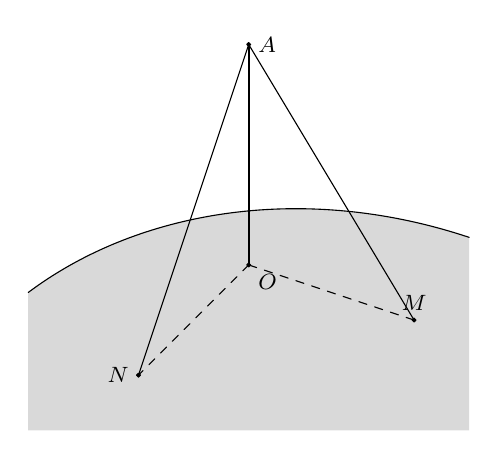
\begin{tikzpicture}[scale=0.7, font=\footnotesize, line join=round, line cap=round, >=stealth]
			\coordinate (O) at (0,0);
			\coordinate (A) at (0,4);
			\coordinate (M) at (3,-1);
			\coordinate (N) at (-2,-2);
			\draw[fill=gray!30, draw=none] (-4,-0.5) .. controls (-2,1) and (1,1.5) .. (4,0.5) -- (4,-3) -- (-4,-3) -- cycle;
			\draw (-4,-0.5) .. controls (-2,1) and (1,1.5) .. (4,0.5);
			\draw[thick] (O) -- (A);
			\draw (A) -- (M);
			\draw (A) -- (N);
			\draw[dashed] (O) -- (M);
			\draw[dashed] (O) -- (N);
			\draw[fill=black] (O) circle (1pt) node[below right] {$O$};
			\draw[fill=black] (A) circle (1pt) node[right] {$A$};
			\draw[fill=black] (M) circle (1pt) node[above] {$M$};
			\draw[fill=black] (N) circle (1pt) node[left] {$N$};
		\end{tikzpicture}
	}
	\loigiai{
		\begin{enumerate}
			\item[a)] Ta có $\overrightarrow{MA}=(0-3;0-(-4);6-3)=(-3;4;3)$ và $\overrightarrow{NA}=(0-(-5);0-(-2);6-2)=(5;2;4)$.\\
			Độ dài dây cáp $MA=\sqrt{(-3)^2+4^2+3^2}=\sqrt{34}\approx 5{,}8$ m.\\
			Độ dài dây cáp $NA=\sqrt{5^2+2^2+4^2}=\sqrt{45}=3\sqrt{5}\approx 6{,}7$ m.
			\item[b)] Mặt phẳng sườn đồi là mặt phẳng $(OMN)$.\\
			Ta có $\overrightarrow{OM}=(3;-4;3)$ và $\overrightarrow{ON}=(-5;-2;2)$.\\
			Véc-tơ pháp tuyến của mặt phẳng $(OMN)$ là $\overrightarrow{n}=\left[\overrightarrow{OM},\overrightarrow{ON}\right]=(-2;-21;-26)$.\\
			Gọi $\alpha$, $\beta$ lần lượt là góc tạo bởi $MA$, $NA$ với mặt phẳng $(OMN)$.
			\begin{itemize}
				\item $\sin\alpha = \dfrac{\left|\overrightarrow{MA}\cdot\overrightarrow{n}\right|}{\left|\overrightarrow{MA}\right|\cdot\left|\overrightarrow{n}\right|} = \dfrac{|(-3)(-2)+4(-21)+3(-26)|}{\sqrt{34}\cdot\sqrt{(-2)^2+(-21)^2+(-26)^2}} = \dfrac{|-156|}{\sqrt{34}\sqrt{1\,121}}=\dfrac{156}{\sqrt{38\,114}} \Rightarrow \alpha \approx 53^\circ$.
				\item $\sin\beta = \dfrac{\left|\overrightarrow{NA}\cdot\overrightarrow{n}\right|}{\left|\overrightarrow{NA}\right|\cdot\left|\overrightarrow{n}\right|} = \dfrac{|5(-2)+2(-21)+4(-26)|}{\sqrt{45}\cdot\sqrt{1\,121}} = \dfrac{|-156|}{\sqrt{45}\sqrt{1\,121}}=\dfrac{156}{\sqrt{50\,445}} \Rightarrow \beta \approx 44^\circ$.
			\end{itemize}
		\end{enumerate}
	}
\end{vd}
\begin{vd}%[2H5C2-4]%[Dự án đề cương 3 Khối NH24-25-Dot 1-Viet Hoang Pham]
	Cho hình chóp $S.ABCD$ có đáy $ABCD$ là hình vuông cạnh bằng $10$. Cạnh bên $SA$ vuông góc với mặt phẳng $(ABCD)$ và $SC=10\sqrt{5}$. Gọi $M$, $N$ lần lượt là trung điểm của $SA$ và $CD$. Tính khoảng cách $\mathrm{d}$ giữa $BD$ và $MN$.
	\loigiai{
	\begin{center}
		\begin{tikzpicture}[scale=1, font=\footnotesize, line join=round, line cap=round, >=stealth]
			\coordinate (A) at (0,0,0);
			\coordinate (B) at (0,0,2);
			\coordinate (C) at (2,0,2);
			\coordinate (D) at (2,0,0);
			\coordinate (S) at (0,2,0);
			\coordinate (M) at ($(S)!0.5!(A)$);
			\coordinate (N) at ($(C)!0.5!(D)$);
			\draw[->] (B) -- ($(B)+(0,0,1)$) node[below] {$x$};
			\draw[->] (D) -- ($(D)+(1,0,0)$) node[right] {$y$};
			\draw[->] (S) -- ($(S)+(0,1,0)$) node[above] {$z$};
			\draw (S)--(B)--(C)--(S);
			\draw (S)--(D);
			\draw (C)--(D);
			\draw[dashed] (A)--(B);
			\draw[dashed] (A)--(D);
			\draw[dashed] (B)--(D);
			\draw[dashed] (A)--(S);
			\draw[dashed] (M)--(N);
			\node[left] at (A) {$A$};
			\node[below] at (B) {$B$};
			\node[below] at (C) {$C$};
			\node[below] at (D) {$D$};
			\node[left] at (S) {$S$};
			\node[above left] at (M) {$M$};
			\node[below] at (N) {$N$};
			\foreach \x in {A,B,C,D,S,M,N}{
			\draw[fill=black] (\x) circle (1pt);
			}
		\end{tikzpicture}
	\end{center}
		Đáy là hình vuông cạnh $10$ nên $AC=\sqrt{10^2+10^2}=10\sqrt{2}$.\\
		Xét tam giác vuông $SAC$ có $SA=\sqrt{SC^2-AC^2}=\sqrt{(10\sqrt{5})^2-(10\sqrt{2})^2}=\sqrt{500-200}=\sqrt{300}=10\sqrt{3}$.\\
		Chọn hệ trục tọa độ như hình vẽ, với $A$ là gốc tọa độ.\\
		Ta có $A(0;0;0)$, $B(10;0;0)$, $D(0;10;0)$, $C(10;10;0)$, $S(0;0;10\sqrt{3})$.\\
		$M$ là trung điểm $SA$ nên $M(0;0;5\sqrt{3})$.\\
		$N$ là trung điểm $CD$ nên $N(5;10;0)$.\\
		Véc-tơ chỉ phương của $MN$ là $\overrightarrow{MN}=(5;10;-5\sqrt{3})\Rightarrow \overrightarrow{u}_1=(1;2;-\sqrt{3})$.\\
		Véc-tơ chỉ phương của $BD$ là $\overrightarrow{BD}=(-10;10;0)\Rightarrow \overrightarrow{u}_2=(-1;1;0)$.\\
		Tích có hướng $\left[\overrightarrow{u}_1,\overrightarrow{u}_2\right]=(\sqrt{3};\sqrt{3};3)$.\\
		Ta có $\overrightarrow{ND}=(-5;0;0)$.\\
		Khoảng cách giữa hai đường thẳng $BD$ và $MN$ là
		\[\mathrm{d}(BD,MN)=\dfrac{\left|\left[\overrightarrow{u}_1,\overrightarrow{u}_2\right]\cdot\overrightarrow{ND}\right|}{\left|\left[\overrightarrow{u}_1,\overrightarrow{u}_2\right]\right|}=\dfrac{|\sqrt{3}(-5)+\sqrt{3}(0)+3(0)|}{\sqrt{(\sqrt{3})^2+(\sqrt{3})^2+3^2}}=\dfrac{5\sqrt{3}}{\sqrt{15}}=\sqrt{5}.\]
	}
\end{vd}
%-----------------------------------------------------------------------------
\subsection{BÀI TẬP RÈN LUYỆN}
\ind{PHẦN I.} \inden{Câu trắc nghiệm nhiều phương án lựa chọn. Mỗi câu hỏi học sinh chỉ chọn một phương án.}\\
\setcounter{ex}{0}
\Opensolutionfile{ans}[ans/2H5-B2-TN]

\begin{ex}%[2H5N2-2]
[Trích đề số 1 minh họa THPTQG - Năm học 2024-2025]
	Trong không gian với hệ tọa độ $Oxyz$, cho hai điểm $A(1;1;2)$, $B(2;-1;3)$. Phương trình đường thẳng $AB$ là
	\choice
	{$\dfrac{x-1}{3}=\dfrac{y-1}{2}=\dfrac{z-2}{1}$}
	{\True $\dfrac{x-1}{1}=\dfrac{y-1}{-2}=\dfrac{z-2}{1}$}
	{$\dfrac{x-3}{1}=\dfrac{y+2}{1}=\dfrac{z-1}{2}$}
	{$\dfrac{x+1}{3}=\dfrac{y+1}{-2}=\dfrac{z+2}{1}$}
	\loigiai{
		Ta có $\overrightarrow{AB}=(2-1; -1-1; 3-2) = (1;-2;1)$.\\
		Đường thẳng $AB$ đi qua điểm $A(1;1;2)$ và nhận véc-tơ $\overrightarrow{AB}=(1;-2;1)$ làm véc-tơ chỉ phương.\\
		Vậy phương trình của $AB$ là $\dfrac{x-1}{1}=\dfrac{y-1}{-2}=\dfrac{z-2}{1}$.
	}
\end{ex}

\begin{ex}%[2H5N2-2]
[Trích đề số 2 minh họa THPTQG - Năm học 2024-2025]
	Trong không gian với hệ tọa độ $Oxyz$, cho điểm $M(1;2;3)$. Gọi $M_1$, $M_2$ lần lượt là hình chiếu vuông góc của $M$ lên các trục $Ox$, $Oy$. Vectơ nào dưới đây là một véctơ chỉ phương của đường thẳng $M_1M_2$?
	\choice
	{$\overrightarrow{u}_1=(0;2;0)$}
	{$\overrightarrow{u}_2=(1;2;0)$}
	{$\overrightarrow{u}_3=(1;0;0)$}
	{\True $\overrightarrow{u}_4=(-1;2;0)$}
	\loigiai{
		$M_1$ là hình chiếu của $M$ lên trục $Ox$ nên $M_1(1;0;0)$.\\
		$M_2$ là hình chiếu của $M$ lên trục $Oy$ nên $M_2(0;2;0)$.\\
		Khi đó $\overrightarrow{M_1M_2}=(-1;2;0)$ là một vectơ chỉ phương của $M_1M_2$.
	}
\end{ex}

\begin{ex}%[2H5H2-3]
[Trích đề số 3 minh họa THPTQG - Năm học 2024-2025]
    Trong không gian $Oxyz$, phương trình của đường thẳng đi qua $M\left( 1;2;1 \right)$ và $N\left( 3;1;-2 \right)$ là
    \choice
    {$\dfrac{x+1}{4}=\dfrac{y+2}{3}=\dfrac{z+1}{-1}$}
    {\True $\dfrac{x-1}{2}=\dfrac{y-2}{-1}=\dfrac{z-1}{-3}$}
    {$\dfrac{x-1}{4}=\dfrac{y-2}{3}=\dfrac{z-1}{-1}$}
    {$\dfrac{x+1}{2}=\dfrac{y+2}{-1}=\dfrac{z+1}{-3}$}
    \loigiai{
    Ta có đường thẳng $MN$ đi qua $M\left( 1;2;1 \right)$ và nhận vectơ $\overrightarrow{MN}=\left( 2;-1;-3 \right)$ làm vectơ chỉ phương nên có phương trình 
    $$\dfrac{x-1}{2}=\dfrac{y-2}{-1}=\dfrac{z-1}{-3}.$$
    }
\end{ex}

\begin{ex}%[2H5H2-3]
[Trích đề số 4 minh họa THPTQG - Năm học 2024-2025]
	Trong không gian $Oxyz$, phương trình của đường thẳng đi qua $A(-1; -1; 1)$ và có một vectơ chỉ phương $\overrightarrow{u} = (1; 2; 3)$ là:
	\choice
	{$\dfrac{x - 1}{1} = \dfrac{y - 1}{2} = \dfrac{z + 1}{3}$}
	{$\dfrac{x + 1}{-1} = \dfrac{y + 2}{-1} = \dfrac{z + 3}{1}$}
	{\True $\dfrac{x + 1}{1} = \dfrac{y + 1}{2} = \dfrac{z - 1}{3}$}
	{$\dfrac{x - 1}{-1} = \dfrac{y - 2}{-1} = \dfrac{z - 3}{1}$}
	\loigiai{
		Phương trình chính tắc của đường thẳng đi qua là $A(-1; -1; 1)$ và có vectơ chỉ phương  $\overrightarrow{u} = (1; 2; 3)$ là
		\[
		\dfrac{x + 1}{1} = \dfrac{y + 1}{2} = \dfrac{z - 1}{3}.
		\]
	}
\end{ex}

\begin{ex}%[2H5H2-2]
[Trích đề số 5 minh họa THPTQG - Năm học 2024-2025]
	Trong không gian $Oxyz$, cho đường thẳng $d\colon \dfrac{x - 1}{2} = \dfrac{y - 3}{-5} = \dfrac{z + 2}{3}$.
	Vectơ nào dưới đây là một vectơ chỉ phương của đường thẳng $d$?
	\choice
	{$\overrightarrow{u} = (2; 5; 3)$}
	{$\overrightarrow{u} = (1; 3; 2)$}
	{$\overrightarrow{u} = (1; 3; -2)$}
	{\True $\overrightarrow{u} = (2; -5; 3)$}
	\loigiai{
		Vectơ chỉ phương của đường thẳng $d$ là $\overrightarrow{u}=(2;-5;3)$.
	}
\end{ex}

\begin{ex}%[2H5N2-3]
[Trích đề số 6 minh họa THPTQG - Năm học 2024-2025]
Trong không gian $Oxyz$, phương trình của đường thẳng đi qua điểm $M(1;-3;5)$ và có một vectơ chỉ phương $\overrightarrow{u}=(2;-1;1)$ là
\choice
{$\dfrac{x-1}{2} = \dfrac{y+3}{-1} = \dfrac{z-5}{1}$}
{$\dfrac{x+1}{2} = \dfrac{y+3}{-1} = \dfrac{z+5}{1}$}
{\True $\dfrac{x-1}{2} = \dfrac{y+3}{1} = \dfrac{z-5}{-1}$}
{$\dfrac{x+1}{2} = \dfrac{y+3}{-1} = \dfrac{z-5}{-1}$}
\loigiai{
Phương trình của đường thẳng đi qua điểm $M(1;-3;5)$ và có một vectơ chỉ phương $\overrightarrow{u}=(2;-1;1)$ là $\dfrac{x-1}{2} = \dfrac{y+3}{1} = \dfrac{z-5}{-1}$.
}
\end{ex}

\begin{ex}%[2H5H2-3]
[Trích đề số 7 minh họa THPTQG - Năm học 2024-2025]
Trong không gian $Oxyz$, cho mặt phẳng $(P)\colon 2x-y-2z+3=0$. Đường thẳng $\Delta$ đi qua điểm $M(4;1;-3)$ và vuông góc $(P)$ với có phương trình chính tắc là
\choice
{$\dfrac{x+4}{2}=\dfrac{y+1}{-1}=\dfrac{z-3}{-2}$}
{$\dfrac{x-2}{4}=\dfrac{y+1}{1}=\dfrac{z+2}{-3}$}
{$\dfrac{x+2}{2}=\dfrac{y+2}{1}=\dfrac{z-3}{-2}$}
{\True $\dfrac{x-4}{2}=\dfrac{y-1}{-1}=\dfrac{z+3}{-2}$}
\loigiai{
Ta có $\Delta \perp (P) \Rightarrow $ VTCP $\overrightarrow{u}_{\Delta}=(2;-1;-2)$.\\
Khi đó, đường thẳng $\Delta$ đi qua điểm $M(4;1;-3)$ và vuông góc $(P)$ có phương trình chính tắc là
\[\dfrac{x-4}{2}=\dfrac{y-1}{-1}=\dfrac{z+3}{-2}.\]
}
\end{ex}

\begin{ex}%[2H5N2-5]
[Trích đề số 8 minh họa THPTQG - Năm học 2024-2025]
	Trong không gian $Oxyz$, đường thẳng $\Delta\colon \dfrac{x-1}{1}=\dfrac{y-1}{-1}=\dfrac{z}{-1}$ song song với mặt phẳng nào sau đây?
	\choice
	{$(P)\colon x+y-z=0$}
	{\True $(\beta)\colon x+z=0$}
	{$(Q)\colon x+y+2z=0$}
	{$(\alpha)\colon x-y+1=0$}
	\loigiai{
		Đường thẳng $\Delta$ có $\overrightarrow{u}=(1;-1;-1)$ là một vectơ chỉ phương và $M(1;1;0)\in\Delta$.\\
		Mặt phẳng $(\beta)$ có $\overrightarrow{n}_{(\beta)}=(1;0;1)$ là một vectơ pháp tuyến.\\
		Ta có $\overrightarrow{u}\cdot\overrightarrow{n}_{(\beta)}=0$ nên $\overrightarrow{u}\perp\overrightarrow{n}_{(\beta)}$.\\
		Đồng thời điểm $M(1;1;0)\notin(\beta)$.\\
		Vậy $\Delta\parallel(\beta)$.
	}
\end{ex}

\begin{ex}%[2H5N2-3]
[Trích đề Moon số 1 minh họa THPTQG - Năm học 2024-2025]
	Trong không gian $Oxyz$, đường thẳng đi qua hai điểm $\mathrm{P}(1;-1;2)$ và $Q(2;0;1)$ có phương trình tham số là
	\choice
	{\True $\heva{&x=2+t\\ &y=t\\ &z=1-t}$}
	{$\heva{&x=1+t\\ &y=-1+t\\ &z=2+t}$}
	{$\heva{&x=2-t\\ &y=t\\ &z=1+t}$}
	{$\heva{&x=1+t\\ &y=-1-t\\ &z=2+t}$}
	\loigiai{
		Phương trình đường thẳng đi qua điểm $Q(2;0;1)$ có vectơ chỉ phương $\overrightarrow{PQ}=(1;1;-1)$ là 
		\[\heva{&x=2+t\\ &y=t\\ &z=1-t}\quad (t\in\mathbb{R}).\]
	}
\end{ex}

\begin{ex}%[2H5N2-3]%[Đề số 27 - Đề thi thử Moon - Đoàn Minh Tâm]
[Trích đề Moon số 27 minh họa THPTQG - Năm học 2024-2025 ]
 	Cho tứ diện đều $ ABCD$ cạnh $ a$. Góc giữa hai véc-tơ $\overrightarrow{AB}$ và $\overrightarrow{CD}$ bằng
 	\choice
 	{$30^\circ$}
 	{\True $90^\circ$}
 	{$60^\circ$}
 	{$45^\circ$}
 	\loigiai{
 		\immini{
 		Gọi $ M $ là trung điểm của đoạn thẳng CD.\\
 		Vî $ ABCD $ là tứ diện đều nên $ BCD $ và $ ACD $ là các tam giác đều.\\
 		Suy ra $\heva{&{AM\perp CD}\\&{BM\perp CD}.}$\\
 		Dẫn đến $ CD\perp\left(ABM\right)$, mà $ AB\subset\left(ABM\right)$ nên $ CD\perp AB$.\\
 		Do đó $\overrightarrow{CD}\perp\overrightarrow{AB}$.\\
 		Vậy $\left(\overrightarrow{CD},\overrightarrow{AB}\right)=90^\circ$.}{
			 \begin{tikzpicture}[line join=round,line cap=round,line width=.6pt,font=\footnotesize,scale=.6]
			 	\coordinate[label=left:$B$] (A) at (0,0);
			 	\coordinate[label=below:$C$] (B) at (1,-1);
			 	\coordinate[label=right:$D$] (C) at (4,0);
			 	\coordinate[label=below right:$M$] (M) at ($(B)!.5!(C)$);
			 	\coordinate (O) at ($(A)!2/3!(M)$);
			 	\coordinate[label=above:$A$] (S) at ($(O)+(90:4)$);
			 	\draw (A)--(B)--(C)--(S)--cycle (S)--(B)  (S)--(M);
			 	\draw[dashed] (M)--(A)--(S) (A)--(C);
			 	\fill (A)circle(1.5pt) (B)circle(1.5pt) (C)circle(1.5pt) (S)circle(1.5pt) (M)circle(1.5pt);
			 \end{tikzpicture}

		 }}
 \end{ex}

\begin{ex}%[2H5H2-3]%[Đề số 27 - Đề thi thử Moon - Đoàn Minh Tâm]
[Trích đề Moon số 27 minh họa THPTQG - Năm học 2024-2025]
 	Trong không gian $ Oxyz$, cho hai điểm $ A\left(-1;2;3\right)$ và $ B\left(3;-2;1\right)$. Phương trình đường trung tuyến $ OM$ của tam giác $ OAB$ là
 	\choice
 	{$\heva{&{x=4t}\\&{y=-4t}\\&{z=2t}}$}
 {$\heva{&{x=4t}\\&{y=-4t}\\&{z=-2t}}$}
{\True $\heva{&	{x=t}\\&{y=0}\\&{z=2t}}$}
{$\heva{&{x=2t}\\&{y=0}\\&{z=-4t}}$}
\loigiai{
Điểm $ M$ là trung điểm của $ AB$ nên tọa độ của $ M$ là $\left(1;0;2\right)$, suy ra $\overrightarrow{OM}=\left(1;0;2\right)$.\\
Phương trình đường thẳng đi qua $ O\left(0;0;0\right)$ và nhận $\overrightarrow{OM}=\left(1;0;2\right)$ làm một véc-tơ chỉ phương là $\heva{&{x=t}\\&{y=0}\\&{z=2t}.}$}
 \end{ex}

\begin{ex}%[DuAnC-dot4, Lê Minh Thiện Anh]%[2H5N2-3]
[Trích đề Moon số 28 minh họa THPTQG - Năm học 2024-2025 ]
	Trong không gian $Oxyz$, cho mặt phẳng $(P)\colon 2x-3y-z-4=0$. Phương trình nào dưới đây là phương trình tham số của đường thẳng đi qua điểm $I(-1;0;2)$ và vuông góc với $(P)$?
	\choice
	{$\heva{&x=1-2t \\&y=3t \\&z=2+t}$}
	{\True $\heva{&x=-1+2t \\	&y=-3t \\&z=2-t}$}
	{$\heva{&x=2+t \\&y=-3\\&z=-1-2t}$}
	{$\heva{&x=2-t \\&y=-3\\&z=-1+2t}$}
	\loigiai{
	$(P)$	 có một véc-tơ pháp tuyến là $\overrightarrow{n}=(2;-3;-1)$.\\
	Gọi $d$ là đường thẳng qua $I(-1;0;2)$ và vuông góc với $(P)$. Ta có $\overrightarrow{u}_d=\overrightarrow{n}_P=(2;-3;-1)$.\\
	$d\colon \heva{&x=-1+2t \\	&y=-3t \\&z=2-t.}$
}
\end{ex}

\begin{ex}%[Dự án C THPTQG 2025]%[Đoàn Thanh Phong]%%[2H5H2-3]
[Trích đề Moon số 29 minh họa THPTQG - Năm học 2024-2025]
	Trong không gian $Oxyz$, cho mặt phẳng $(P)\colon x - 2y + 3z - 4 = 0$. Đường thẳng $d$ đi qua gốc tọa độ $O$ và vuông góc với $(P)$ có một vectơ chỉ phương là
	\choice
	{ $\overrightarrow{u}_1 = (-1;-2;3)$ } 
	{ $\overrightarrow{u}_2 = (1;2;3)$ }
	{\True $\overrightarrow{u}_3 = (-1;2;-3)$ }
	{ $\overrightarrow{u}_4 = (1;-2;-3)$ }
	\loigiai{
		Mặt phẳng $(P)\colon x - 2y + 3z - 4 = 0$ có một vectơ  pháp tuyến là $\overrightarrow{n}_P = (1; -2; 3)$.\\
		Vì $d\perp (P)$ nên $\overrightarrow{u}_d=\overrightarrow{n}_P = (1; -2; 3)$ là một vectơ  chỉ phương.\\
		Do đó, $\overrightarrow{u} = -(-1; 2; -3)$ cũng là một vectơ  chỉ phương của $d$. 
	}
\end{ex}

\begin{ex}%[Dự án C THPTQG 2025]%[Đoàn Thanh Phong]%[2H5H2-7]
[Trích đề Moon số 29 minh họa THPTQG - Năm học 2024-2025]
	\immini{Cho tứ diện $OABC$ có $OA, OB, OC$ đôi một vuông góc với nhau và $OA = OB = OC = a\sqrt{3}$.
		Góc giữa hai vectơ $\overrightarrow{AB}$ và $\overrightarrow{BC}$ bằng
		\choice
		{ $60^\circ$ }
		{\True $120^\circ$ }
		{ $90^\circ$ }
		{ $45^\circ$ }}{
		\begin{tikzpicture}[line join=round,line cap=round,line width=.6pt,font=\footnotesize,scale=.8]
			\coordinate[label=left:$O$] (O) at (0,0);
			\coordinate[label=below:$B$] (B) at (-1,-1);
			\coordinate[label=below:$C$] (C) at (3,0);
			\coordinate[label=above left:$A$] (A) at ($(O)+(90:3)$);
			\draw (A)--(B)--(C)--cycle;
			\draw[dashed] (A)--(O)--(C) (O)--(B);
			\draw ($ (O)!5pt!(C)$)--($(O)!2!($($(O)!5pt!(C)$)!.5!($(O)!5pt!(A)$)$)$)--($(O)!5pt!(A)$);
			\fill (O)circle(1.25pt) (B)circle(1.25pt) (C)circle(1.25pt) (A)circle(1.25pt);
		\end{tikzpicture}	
	}
	\loigiai{
		\immini{
			\textbf{Cách 1}: Xét trong mặt phẳng $(ABC)$, dựng $\overrightarrow{AB}=\overrightarrow{BA'}$.\\
			Khi đó $\left(\overrightarrow{AB},\overrightarrow{BC}\right)=\left(\overrightarrow{BA'},\overrightarrow{BC}\right)=\widehat{A'BC}=180^\circ-60^\circ=120^\circ$\\
			\textbf{Cách 2}: Chọn hệ trục tọa độ $Oxyz$ sao cho $O$ là gốc tọa độ, $A(a\sqrt{3}; 0; 0)$, $B(0; a\sqrt{3}; 0)$, $C(0; 0; a\sqrt{3})$.\\
			Ta có
			$\overrightarrow{AB} = (-a\sqrt{3}; a\sqrt{3}; 0)$ và
			$\overrightarrow{BC} = (0; -a\sqrt{3}; a\sqrt{3})$.\\
			Ta có 	$\overrightarrow{AB} \cdot \overrightarrow{BC} = -3a^2$; $|\overrightarrow{AB}| = a\sqrt{6}$ và 
			$|\overrightarrow{BC}| = a\sqrt{6}$.\\
			Gọi $\alpha$ là góc giữa hai vectơ $\overrightarrow{AB}$ và $\overrightarrow{BC}$. \\
			Ta có
			$\cos \alpha= \dfrac{\overrightarrow{AB} \cdot \overrightarrow{BC}}{|\overrightarrow{AB}| \cdot |\overrightarrow{BC}|} = \dfrac{-3a^2}{6a^2} = -\dfrac{1}{2}$.\\
			Vậy $\alpha= 120^\circ$.}{
			\begin{tikzpicture}[line join=round,line cap=round,line width=.6pt,font=\footnotesize,scale=.8]
				\coordinate[label=left:$O$] (O) at (0,0);
				\coordinate[label=below:$B$] (B) at (-1,-1);
				\coordinate[label=below:$C$] (C) at (3,0);
				\coordinate[label=above left:$A$] (A) at ($(O)+(90:3)$);
				\coordinate[label=above left:$x$] (M) at ($(O)!2!(B)$);
				\coordinate[label=above: $y$] (N) at ($(O)!1.5!(C)$);
				\coordinate[label=left:$z$] (P) at ($(O)!1.5!(A)$);
				\draw (A)--(B)--(C)--cycle;
				\draw[dashed] (A)--(O)--(C) (O)--(B);
				\draw[->] (B)--(M);
				\draw[->] (C)--(N);
				\draw[->] (A)--(P);
				\draw ($ (O)!5pt!(C)$)--($(O)!2!($($(O)!5pt!(C)$)!.5!($(O)!5pt!(A)$)$)$)--($(O)!5pt!(A)$);
				\fill (O)circle(1.25pt) (B)circle(1.25pt) (C)circle(1.25pt) (A)circle(1.25pt);
			\end{tikzpicture}	
		}
	}
\end{ex}

\begin{ex}%[Dự Án C- Đề Moon 46 ]%[Nguyễn Văn Sang]%[2H5N2-3]
[Trích đề Moon số 46 minh họa THPTQG - Năm học 2024-2025]
    Trong không gian $Oxyz$, đường thẳng đi qua hai điểm $A(1;1;1)$, $B(-1;2;0)$ có phương trình là
    \choice
    {$\dfrac{x+1}{2} = \dfrac{y+1}{-1} = \dfrac{z+1}{1}$}
    {\True $\dfrac{x-1}{-2} = \dfrac{y-1}{1} = \dfrac{z-1}{-1}$}
    {$\dfrac{x+1}{-2} = \dfrac{y+1}{-1} = \dfrac{z+1}{1}$}
    {$\dfrac{x-1}{-2} = \dfrac{y-1}{-1} = \dfrac{z-1}{1}$}
    \loigiai{
    Vecto chỉ phương của đường thẳng $AB$ là $\overrightarrow{AB} =(-2; 1; -1)$.\\
    Phương trình đường thẳng $AB$ là $\dfrac{x-1}{-2} = \dfrac{y-1}{1} = \dfrac{z-1}{-1}$.
    }
\end{ex}

\begin{ex}%[2H5H2-3]%[Dự án C Đợt 4-Đề thi thử 2025 MOON-48]%[Lê Hùng Thắng]%%Câu 6
[Trích đề Moon số 46 minh họa THPTQG - Năm học 2024-2025]
Trong không gian $Oxyz$, mặt phẳng $(P)$ đi qua $ M\left(1;1;-1\right)$ và vuông góc với đường thẳng $\Delta\colon \dfrac{x+1}{2}=\dfrac{y-2}{2}=\dfrac{z-1}{1}$ có phương trình là
\choice
{$ 2x+2y+z+3=0$}
{\True $ 2x+2y+z-3=0$}
{$ x-2y-z=0$}
{$ x-2y-z-2=0$}
\loigiai{
Mặt phẳng $(P)$ có một vectơ pháp tuyến là $\overrightarrow{n}=\left(2;2;1\right)$.\\
Vậy phương trình mặt phẳng $(P)$ là $2\left(x-1\right)+2\left(y-1\right)+\left(z+1\right)=0\Leftrightarrow 2x+2y+z-3=0$.
}
\end{ex}

\begin{ex}%[2H5H2-3]
[Trích đề Moon số 49 minh họa THPTQG - Năm học 2024-2025]
   Trong không gian $Oxyz$ cho hai điểm $A\left( 1;-2;3 \right)$ và $B\left( 3;1;1 \right)$. Đường thẳng $AB$ có phương trình là
    \choice
    {$\dfrac{x-1}{4}=\dfrac{y+2}{-1}=\dfrac{z-3}{4}$}
    {\True $\dfrac{x-1}{2}=\dfrac{y+2}{3}=\dfrac{z-3}{-2}$}
    {$\dfrac{x-4}{1}=\dfrac{y+1}{-2}=\dfrac{z-4}{3}$}
    {$\dfrac{x-2}{2}=\dfrac{y-3}{-2}=\dfrac{z+2}{3}$}
    \loigiai{
    Ta có $\overrightarrow{AB}=\left( 2;3;-2 \right)$.\\ 
    Suy ra đường thẳng $AB$ có vectơ chỉ phương là $\overrightarrow{u}=\left( 2;3;-2 \right)$.\\
    Mà đường thẳng $AB$ đi qua điểm $A\left( 1;-2;3 \right)$ nên $AB$ có phương trình chính tắc là 
    $$\dfrac{x-1}{2}=\dfrac{y+2}{3}=\dfrac{z-3}{-2}.$$
    }
\end{ex}

\begin{ex}%[TT THPT Lê Thánh Tông, HCM, 24-25]%[Trần Hoà]%[2H5H2-2]
[Trích đề KSCL - THPT Lê Thánh Tông - TP.HCM - Năm học 2024-2025]
	Trong không gian $Oxyz$, cho đường thẳng $d\colon \dfrac{x-1}{4}=\dfrac{-y}{2}=\dfrac{z+2}{-6}$. Vectơ nào dưới đây là một vectơ chỉ phương của $d$?
	\choice
	{$\overrightarrow{u}_{2}=(2;-1;3)$}
	{$\overrightarrow{u}_{1}=(4;2;-6)$}
	{\True $\overrightarrow{u}_{3}=(-2;1;3)$}
	{$\overrightarrow{u}_{4}=(1;0;2)$}
	\loigiai{
		Phương trình đường thẳng $d$ được viết lại là $\dfrac{x-1}{4}=\dfrac{y}{-2}=\dfrac{z+2}{-6}$.\\
		Suy ra tọa độ của một vectơ chỉ phương của $d$ là $(4;-2;-6)$.\\
		Do đó $\overrightarrow{u}_{3}=(-2;1;3)$ cũng là vectơ chỉ phương của $d$.
	}
\end{ex}

\begin{ex}%[2H5N2-2]%[Dự án C - Đợt 4 LocDo]
[Trích đề Moon số 46 minh họa THPTQG - Năm học 2024-2025]
	Trong không gian $Oxy$, cho đường thẳng $d\colon\dfrac{x-1}{4} = \dfrac{-y}{2} = \dfrac{z+2}{-6}$. Vectơ nào dưới đây là một vectơ chỉ phương của $d$?
	\choice
	{$\overrightarrow{u}_2 = (2;-1;3)$}
	{$\overrightarrow{u}_1 = (4;2;-6)$}
	{\True $\overrightarrow{u}_3 = (-2;1;3)$}
	{$\overrightarrow{u}_4 = (1;0;2)$}
	\loigiai{
	 Viết lại phương trình đường thẳng $d\colon\dfrac{x-1}{4}=\dfrac{y}{-2}=\dfrac{z+2}{-6}$.\\
	Suy ra một vectơ chỉ phương của đường thẳng $d$ là $\overrightarrow{u}=(4;-2;-6)=-2\cdot(-2;1;3)$.\\
	Suy ra vectơ $\overrightarrow{u}_3=(-2;1;3)$ cũng là một vectơ chỉ phương của đường thẳng $d$. 
	}
\end{ex}

\begin{ex}%[2H5N2-3]%[Đề số 5-THPT-QG]%[Huỳnh Thanh Chí]
[Trích đề Moon số 5 minh họa THPTQG - Năm học 2024-2025]
	Trong không gian $Oxyz$, phương trình của đường thẳng đi qua $M(1; 2; 1)$ và $N(3; 1;-2)$ là
	\choice
	{$\dfrac{x+1}{4}=\dfrac{y+2}{3}=\dfrac{z+1}{-1}$}
	{\True $\dfrac{x-1}{2}=\dfrac{y-2}{-1}=\dfrac{z-1}{-3}$}
	{$\dfrac{x-1}{4}=\dfrac{y-2}{3}=\dfrac{z-1}{-1}$}
	{$\dfrac{x+1}{2}=\dfrac{y+2}{-1}=\dfrac{z+1}{-3}$}
	\loigiai{
		Ta có đường thẳng $MN$ đi qua $M(1; 2; 1)$ và nhận vectơ $\overrightarrow{MN}=(2;-1;-3)$ làm vectơ chỉ phương nên có phương trình $\dfrac{x-1}{2}=\dfrac{y-2}{-1}=\dfrac{z-1}{-3}$.
	}
\end{ex}


\Closesolutionfile{ans}

\ind{PHẦN II.} \inden{Câu trắc nghiệm đúng sai. Trong mỗi ý a), b), c), d) ở mỗi câu, học sinh chọn đúng hoặc sai.}\\
\setcounter{ex}{0}
\Opensolutionfile{ans}[ans/2H5-B2-DS]%--Đặt tên 2D1-Bai1-DS


\begin{ex}%[2H5V2-7]%[Dự án đề kiểm tra Toán 12 HKII NH25-26- Phạm Văn Long]%[THPT - CHUYÊN LÊ HỒNG PHONG - TPHCM]
[Trích đề HKII - THPT CHUYÊN LÊ HỒNG PHONG - TPHCM - NH 2024-2025]
	Trong không gian $Oxyz$, cho dường thẳng $\Delta\colon \dfrac{x-1}{2}=\dfrac{y-1}{1}=\dfrac{z-2}{3}$ và mặt phẳng $(P)\colon x-y+z-2024=0$.
	\choiceTF
	{\True Véc-tơ có tọa độ $(2;1;3)$ là một véc-tơ chỉ phương của $\Delta$}
	{Véc-tơ có tọa độ $(1;1;2)$ là một véc-tơ pháp tuyến của $(P)$}
	{Cô-sin của góc giữa hai véc-tơ $\vec{u}=(-5; 12;-13)$ và $\vec{n}=(1;2;2)$ bằng $\dfrac{7}{39\sqrt{2}}$}
	{\True Góc giữa hai đường thẳng $\Delta$ và mặt phẳng $(P)$ (làm tròn đến hàng đơn vị của độ) bằng $38^{\circ}$}
	\loigiai{
		\begin{itemchoice}
			\itemch 
			Một véc-tơ chỉ phương của $\Delta$ là $\overrightarrow{u}=(2;1;3)$.
			\itemch 
			Một véc-tơ pháp tuyến của $(P)$ là $\overrightarrow{n}=(1;-1;1)$.
			\itemch 
			$\cos \left(\vec{u},\vec{n}\right)=\dfrac{-5\cdot 1+12\cdot 2+(-13)\cdot 2}{\sqrt{25+144+169}\cdot \sqrt{1+4+4}}=-\dfrac{7\sqrt{2}}{78}=-\dfrac{7}{39\sqrt{2}}$.
			\itemch 
			$\sin \left(\Delta,(P)\right)=\dfrac{|2\cdot 1+1\cdot (-1)+3\cdot 1|}{\sqrt{4+1+9}\cdot \sqrt{1+1+1}}=\dfrac{2\sqrt{42}}{21}\Rightarrow \left(\Delta,(P)\right)\approx 38^{\circ}$.
		\end{itemchoice}
	}
\end{ex}

\begin{ex}%[2H5V2-5]%[Tran Xuan Hoa]%[THPT Nguyễn Hữu Cầu HK2-NH24-25-HCM]
[Trích đề HKII - THPT Nguyễn Hữu Cầu - TPHCM - NH 2024-2025]
	Trong không gian với hệ trục $Oxyz$, cho mặt phẳng $(P)\colon  2x - y + z - 2 = 0$ và điểm $A(-1; 1; -1)$. Các khẳng định sau đúng hay sai?
	\choiceTF
	{\True Khoảng cách từ $A$ đến mặt phẳng $(P)$ bằng $\sqrt{6}$}
	{\True $\sin$ của góc tạo bởi $OA$ và mặt phẳng $(P)$ bằng $\dfrac{2\sqrt{2}}{3}$}
	{Đường thẳng $\Delta$ qua $A$ và vuông góc với $(P)$ có phương trình $\dfrac{x - 1}{2} = \dfrac{y + 1}{-1} = \dfrac{z - 1}{1}$}
	{$M(a;b;c)$ là điểm thuộc $(P)$ sao cho $AM$ ngắn nhất, ta có $a + b + c = 2$}
	\loigiai{
		Gọi $(P)\colon  2x - y + z - 2 = 0$ có vectơ pháp tuyến $\vec{n} = (2; -1; 1)$, điểm $A(-1; 1; -1)$.		
		\begin{itemchoice}
			\itemch 
			Khoảng cách từ $A$ đến mặt phẳng $(P)$ là
			\[
			d = \dfrac{|2(-1) - 1 + (-1) - 2|}{\sqrt{2^2 + (-1)^2 + 1^2}} = \dfrac{|-2 -1 -1 -2|}{\sqrt{6}} = \dfrac{6}{\sqrt{6}} = \sqrt{6}.
			\]
			\itemch 
			Ta có $\vec{OA} = (-1; 1; -1)$, $\vec{n} = (2; -1; 1)$.\\
			Gọi $\theta$ là góc giữa $OA$ và mặt phẳng $(P)$. Khi đó
			\[
			\sin \theta = \dfrac{|\vec{OA} \cdot \vec{n}|}{|\vec{OA}| \cdot |\vec{n}|} = \dfrac{|(-1)\cdot2 + 1\cdot(-1) + (-1)\cdot1|}{\sqrt{(-1)^2 + 1^2 + (-1)^2} \cdot \sqrt{2^2 + (-1)^2 + 1^2}} = \dfrac{2\sqrt{2}}{3}.
			\]
			\itemch 
			Đường thẳng vuông góc mặt phẳng $(P)$ sẽ có vectơ chỉ phương là $\vec{n} = (2; -1; 1)$ và đi qua $A(-1; 1; -1)$.\\
			Phương trình tham số 
			\[
			\begin{cases}
				x = -1 + 2t\\
				y = 1 - t\\
				z = -1 + t
			\end{cases}
			\Rightarrow \dfrac{x + 1}{2} = \dfrac{y - 1}{-1} = \dfrac{z + 1}{1}.
			\]
			\itemch 
			Điểm $M$ trên $(P)$ sao cho $AM$ ngắn nhất chính là hình chiếu vuông góc từ $A$ lên mặt phẳng $(P)$.\\
			Vì mặt phẳng có dạng $2x - y + z - 2 = 0$, thì tọa độ $M$ thỏa mãn $2a - b + c = 2$.\\
			Khi đó, do $AM$ vuông góc với mặt phẳng nên $AM$ có phương là $\vec{n} = (2; -1; 1)$ và đi từ $A(-1; 1; -1)$ đến $M$.\\
			Gọi $\vec{AM}=k\vec{n} $ nên $M(-1 + 2k; 1 - k; -1 + k)$. Thay vào phương trình mặt phẳng
			\[
			2(-1 + 2k) - (1 - k) + (-1 + k) = 2 \Rightarrow k = 1.
			\]
			Suy ra $M = (-1 + 2; 1 - 1; -1 + 1) = (1; 0; 0)$. Vậy $a+b+c=1\neq 2$.
		\end{itemchoice}
	}
\end{ex}

\begin{ex}%[2H5H2-3]
Trong không gian $Oxyz$, cho hai điểm $A(0;2;-1)$, $B(2;2;-1)$ và đường thẳng\\
 $\Delta \colon \heva{&x=1+2t\\& y=3+t\\& z=4-5t} (t\in\mathbb{R}).$
\choiceTF
{Một vectơ chỉ phương của đường thẳng $\Delta$ là $\vec{u}=(1;3;4)$}
{Phương trình mặt cầu đường kính $AB$ là $(x-1)^2+(y+2)^2+(z-1)^2=2$}
{\True Phương trình chính tắc của đường thẳng $d$ đi qua điểm $A$ và song song với đường thẳng $\Delta$ là $\dfrac{x}{2}=\dfrac{y+2}{1}=\dfrac{z-1}{-5}$}
{Gọi $\alpha$ là góc giữa hai đường thẳng $\Delta$ và $AB$, khi đó $\cos\alpha=\dfrac{\sqrt{30}}{15}$}
\loigiai{
\begin{itemchoice}
\itemch Vectơ chỉ phương của $\Delta$ là $\vec{u}=(2;1;-5)$.
\itemch Gọi $I(1;2;-1)$ là trung điểm $AB$. Khi đó  $\left|\overrightarrow{IA}\right|=\sqrt{(0-1)^2+(2-2)^2+(-1+1)^2}=1$.\\
Phương trình mặt cầu đường kính $AB$ là $(x-1)^2+(y-2)^2+(z+1)^2=1$.
\itemch Phương trình chính tắc của đường thẳng  $d$ có dạng $\dfrac{x}{2}=\dfrac{y-2}{2}=\dfrac{z+1}{-5}$.
\itemch $\cos\left(\Delta, AB\right)=\cos\left(\overrightarrow{AB},\vec{u}_{\Delta}\right)=\dfrac{|2\cdot2+0\cdot1+0\cdot(-5)|}{\sqrt{2^2+0^2+0^2}\cdot\sqrt{2^2+1^2+(-5)^2}}=\dfrac{\sqrt{30}}{30}$.  
\end{itemchoice}
}
\end{ex}

\begin{ex}%[2H5H2-7]%[1-TN-HH-DT-THPT-CheLanVien-QuangTri-HKII-NH24-25]
[Trích đề HKII - THPT Chế Lan Viên - Quảng Trị - NH 2024-2025]
Trong không gian $Oxyz$, cho đường thẳng $\Delta\colon \heva{&x = 2 + t \\&y = 1 - 2t \\&z = 3 + 2t}$ và hai điểm $M(1;1;2)$, $N(-2;3;-2)$.
\choiceTF
{\True Đường thẳng $\Delta$ có vectơ chỉ phương là $\overrightarrow{u} = (1;-2;2)$}
{\True Ta có $\overrightarrow{NM}=(3;-2;4)$.\\
Đường thẳng $MN$ đi qua điểm $M$, có một vectơ chỉ phương $\overrightarrow{NM}=(3;-2;4)$ nên có phương trình chính tắc là $\dfrac{x - 1}{3} = \dfrac{y - 1}{-2} = \dfrac{z - 2}{4}$}
{Mặt cầu $(S)$ tâm $M$ và bán kính $MN$ có phương trình là $(x - 1)^2 + (y - 1)^2 + (z - 2)^2 = 21$}
{Cosin của góc tạo bởi đường thẳng $\Delta$ và đường thẳng $MN$ bằng $\dfrac{5\sqrt{21}}{7}$}
\loigiai
{\begin{itemchoice}
\itemch  So với tham số, hệ số của $t$ chính là vectơ chỉ phương.
\itemch  Phương trình chính tắc phải dùng điểm trên $\Delta\colon \dfrac{x - 2}{1} = \dfrac{y + 1}{-2} = \dfrac{z - 3}{2}$.
\itemch  Ta có $MN^2 = (1 + 2)^2 + (1 - 3)^2 + (2 + 2)^2 = 9 + 4 + 16 = 29$. \\
Suy ra phương trình mặt cầu $(S)$ tâm $M$ và bán kính $MN$ có phương trình là $(x - 1)^2 + (y - 1)^2 + (z - 2)^2 = 29$.
\itemch 
Đường thẳng $\Delta$ và $MN$ có các vectơ chỉ phương lần lượt là $\overrightarrow{u} = (1;-2;2)$ và $\overrightarrow{NM} = (3;-2;4)$.\\
Gọi $\alpha$ là số đo của góc giữa $\Delta$ và $MN$, ta có\\
$\cos \alpha = \dfrac{\big|\overrightarrow{u} \cdot \overrightarrow{NM}\big|}{\big|\overrightarrow{u}\big| \cdot \big|\overrightarrow{NM}\big|} = \dfrac{\big|1\cdot3 + (-2)\cdot(-2) + 2\cdot4\big|}{\sqrt{1^2+(-2)^2+2^2} \cdot \sqrt{3^2+(-2)^2+4^2}} = \dfrac{15}{3\sqrt{29}}\neq \dfrac{5\sqrt{21}}{7}$.
\end{itemchoice}
}
\end{ex}



\begin{ex}%[2H5V2-4]%[2-TN-DS-TLN-SGD-CanTho-HKII-NH24-25]%[Sỹ Trường]
[Trích đề HKII - SGD Cần Thơ - NH 2024-2025]
	Trong không gian $Oxyz$, cho hai đường thẳng $\Delta_1: \dfrac{x}{1}=\dfrac{y+3}{2}=\dfrac{z-2}{3}$ và $\Delta_2: \dfrac{x-5}{2}=\dfrac{y}{4}=\dfrac{z+2}{-1}$.
	\choiceTF
	{\True Gọi $\alpha$ là góc giữa hai đường thẳng $\Delta_1$ và $\Delta_2$. Giá trị của $\cos \alpha$ bằng $\dfrac{\sqrt{6}}{6}$}
	{\True Phương trình tham số của đường thẳng $\Delta_1$ là $\heva{&x=t \\& y=-3+2 t \\ &z=2+3 t}$}
	{Phương trình mặt phẳng chứa $\Delta_1$ và song song với $\Delta_2$ là $-2 x+y-3=0$}
	{\True Hai đường thẳng $\Delta_1$ và $\Delta_2$ chéo nhau}
\loigiai{
	\begin{itemchoice}
		\itemch Ta có $\cos \alpha=\dfrac{|1.2+2.4+3.(-1)|}{\sqrt{1^2+2^2+3^2} \cdot \sqrt{2^2+4^2+(-1)^2}}=\dfrac{\sqrt{6}}{6}$.
		\itemch Ta có $M(0;-3; 2) \in \Delta_1, \overrightarrow{u_1}=(1; 2; 3)$ là một VTCP của $\Delta_1$.\\
		Do đó phương trình tham số của đường thẳng $\Delta_1$ là $\heva{&x=t \\ &y=-3+2 t \\ &z=2+3 t}$.
		\itemch Gọi $(P)$ là mặt phẳng chứa $\Delta_1$ và song song với $\Delta_2$.\\
		Ta có một vectơ pháp tuyến của $ P $ là $ \overrightarrow{n}_{(P)}=\left[\overrightarrow{u}_{\Delta_1},\overrightarrow{u}_{\Delta_2}\right]=(-14; 7; 0) $.\\
		Mặt khác $M(0;-3; 2) \in(P)$ nên phương trình của mặt phẳng $ (P) $ là $$-14(x-0)+7(y+3)=0 \Leftrightarrow-2 x+y+3=0.$$
		\itemch Ta có $\left[\overrightarrow{u_1} \cdot \overrightarrow{u_2}\right] \cdot \overrightarrow{M M_1}=(-14) \cdot 5+7 \cdot 3+0 \cdot(-4)=-49 \neq 0$.\\
		Vậy đường thẳng $\Delta_1$ và $\Delta_2$ chéo nhau.
	\end{itemchoice}
}
\end{ex}

\begin{ex}%[2H5H2-7]%[Dự án đề kiểm tra Toán 12 HKII NH24-25- Phan Anh]%[SGD Kiên Giang]
[Trích đề HKII - SGD Kiên Giang - NH 2024-2025]
	Trong không gian $Oxyz$, cho hai điểm $B(1;2;-1)$, $C(0;2;3)$ và mặt phẳng $(P)\colon x+3y-2z+1=0$.
	\choiceTF
	{\True Mặt phẳng $(P)$ có véc-tơ pháp tuyến $\vec{n}=(1;3;-2)$}
	{Mặt phẳng $(P)$ đi qua điểm $B$}
	{Mặt phẳng $(Q)$ qua $C$ và song song với $(P)$ có phương trình là $x+3y-2z-12=0$}
	{\True Góc giữa mặt phẳng $(P)$ và đường thẳng $d\colon\dfrac{x-1}{2}=\dfrac{y-2}{3}=\dfrac{z+1}{2}$ (làm tròn kết quả đến hàng đơn vị, theo đơn vị độ) bằng $27^\circ$}
	\loigiai{\begin{itemchoice}
			\itemch Mặt phẳng $(P)$ có véc-tơ pháp tuyến là $\vec{n}=(1;3;-2)$.
			\itemch Thay tọa độ điểm $B$ vào phương trình mặt phẳng $(P)$ ta được
			\[1+3\cdot2-2\cdot(-1)+1=0\Leftrightarrow10=0\text{ (vô lý).}\]
			Vậy mặt phẳng $(P)$ không đi qua điểm $B$.
			\itemch Mặt phẳng $(Q)$ song song với mặt phẳng $(P)$ có dạng $x+3y-2z+m=0$, $m\ne1$.\\
			Do mặt phẳng $(Q)$ đi qua $C$ nên $0+3\cdot2-2\cdot3+m=0\Leftrightarrow m=0$.\\
			Suy ra phương trình mặt phẳng $(Q)$ là $x+3y-2z=0$.
			\itemch Đường thẳng $d$ có véc-tơ chỉ phương là $\vec{u}=(2;3;2)$.\\
			Gọi $\varphi$ là góc giữa đường thẳng $d$ và mặt phẳng $(P)$, ta có
			\[\sin\varphi=\dfrac{\left|\vec{u}\cdot\vec{n}\right|}{\left|\vec{u}\right|\cdot\left|\vec{n}\right|}=\dfrac{|2\cdot1+3\cdot3+2\cdot(-2)|}{\sqrt{4+9+4}\cdot\sqrt{1+9+4}}=\dfrac{7}{\sqrt{238}}.\]
			Vậy góc giữa đường thẳng $d$ và mặt phẳng $(P)$ là $27^\circ$.
	\end{itemchoice}}
\end{ex}
\Closesolutionfile{ans}


\ind{PHẦN III.} \inden{Câu trắc nghiệm trả lời ngắn.}\\
\setcounter{ex}{0}
\Opensolutionfile{ans}[ans/2H5-B2-TLN]%--Đặt tên 2D1-Bai1-DS
\begin{ex}%[Thi thử Moon, đề số 6]%[Trần Hoà, Dự án C, lần 4]%[2H5V2-8]%Câu 19
[Trích đề Moon số 6 minh họa THPTQG - Năm học 2024-2025 ]
\immini{Trong một khu du lịch, người ta cho du khách trải nghiệm thiên nhiên bằng cách đu theo đường trượt zipline (là đường thẳng) từ vị trí $A$ cao $15$ m của tháp một này sang vị trí $B$ cao $10$ m của tháp hai trong khung cảnh tuyệt đẹp xung quanh. Với hệ trục toạ độ $Oxyz$ cho trước (đơn vị: mét), toạ độ của $A$ và $B$ lần lượt là $(3;2{,}5;15)$ và $(21;27{,}5;10)$. Bạn Tuấn đang đứng ở mặt đất vị trí có toạ độ $T(12;21;0)$, hỏi khi du khách ở độ cao bao nhiêu mét trên cáp treo sẽ cách bạn Tuấn một khoảng nhỏ nhất (làm tròn kết quả đến hàng phần mười).\par
	\shortans[]{11,4}}{\begin{tikzpicture}[scale=.7]
		%\draw[opacity=0.2] (-4,-4)grid (4,4);
		\def\a{2.4} \def\b{4} \def\c{4}	 \def\g{-130}
		\draw[->] (0,0)--(7,0)node[below]{$y$};
		\draw[->] (0,0)--(\g:3.5)node[below]{$x$};
		\draw[->] (0,0)--(90:5.5)node[right]{$z$};
		\coordinate (O) at (0,0);
		\coordinate (A') at (1,-1);
		\coordinate (A) at ($(A')+(90:4)$);
		\coordinate (B') at (5,-4);
		\coordinate (B) at ($(B')+(90:2.3)$);
		\draw (A)--(B);
		\coordinate (M) at ($(A)!0.3!(B)$);
		\coordinate (T) at (2.6,-2.6);
	%\draw[,rotate=-20,fill,opacity=0.2,yscale=0.5] (-1,6) circle (3.5);
	\draw[line width = 4pt] (A)--(A') (B)--(B');
	\draw[dashed] (M)--(T);
	\foreach \p/\g in {A/90,B/50,O/180,M/40,T/-90} \draw[fill] (\p) circle(.5pt) node [shift={(\g:.3)}] {$\p$}; 
		\end{tikzpicture}}
\loigiai{
Giả sử bạn Tuấn đang đứng ở vị trí $T$ và $M$ là vị trí của du khách.\\
Khi đó du khách gần bạn Tuấn nhất khi $TM \perp AB$.\\
Ta có $\overrightarrow{AB}= (18;25;-5)$.\\
Phương trình tham số chứa đường zipline là $d\colon \heva{&x = 3 + 18t \\& y = 2{,}5 + 25t \\& z = 15 - 5t}$, $(t \in \mathbb{R})$.\\
Gọi $M(3+18t; 2{,}5+25t; 15-5t)$ ta có $\overrightarrow{TM}= (18t-9; 25t-18{,}5; 15-5t)$.\\
Khi đó $\overrightarrow{TM}\cdot \overrightarrow{AB}= 0 \Rightarrow (18t-9; 25t-18{,}5; 15-5t) \cdot (18; 25; -5) = 0$.\\
Suy ra $t = \dfrac{1399}{1948}$
$\Rightarrow z_M \approx 11{,}4$ (m).}
\end{ex}

\begin{ex}%[Dự án đề thi các sở]%Mui Doan]%[2H5H2-7]
[Trích đề Moon số 7 minh họa THPTQG - Năm học 2024-2025]
	Cho hình lăng trụ đứng $ABC.A'B'C'$ có đáy $ABC$ là tam giác vuông tại $C$, $AC=3a$, $BC=4a$ và góc giữa đường thẳng $B'C$ và mặt phẳng $(ABC)$ bằng $45^\circ$. Tính sin của góc giữa đường thẳng $B'C$ và mặt phẳng $(ABC')$ (làm tròn kết quả đến hàng phần trăm).
	\par\shortans{$0{,}73$}
	\loigiai{
		Ta có $CC'\perp (ABC)$ nên $C$ là hình chiếu của $C'$ trên $(ABC)$.\\
		Khi đó $\left(BC',(ABC)\right)=\left(BC',BC\right)=\widehat{C'BC}=45^\circ$.\\
		Xét $\triangle C'BC$ vuông tại $C$, ta có $CC'=BC\tan\widehat{C'BC}=4a\cdot\tan 45^\circ=4a$.\\
		Chọn hệ trục tọa độ $Oxyz$, với $C \equiv O$, $A\in Ox$, $B\in Oy$ và $C'\in Oz$, đơn vị trên các trục là $a$.
		\begin{center}
			\tdplotsetmaincoords{75}{110}
			\begin{tikzpicture}[font=\footnotesize, >=stealth, tdplot_main_coords]
				\path
				(0,0,0) coordinate (C)+(0,0,4) coordinate (C')
				(3,0,0) coordinate (A)+(0,0,4) coordinate (A')
				(0,4,0) coordinate (B)+(0,0,4) coordinate (B')
				;
				\draw (A')--(C')--(B')--cycle (A)--(A') (B)--(B') (A)--(B);
				\draw[dashed] (A)--(C)--(B) (C)--(C') (B')--(C) (A)--(C')--(B);
				\draw[->] (A)--++(3,0,0)node[below]{$x$};
				\draw[->] (B)--++(0,1,0)node[right]{$y$};
				\draw[->] (C')--++(0,0,1)node[left]{$z$};
				\foreach \x/\g in {C/left, A/below, B/below, C'/left, A'/left, B'/right}{
					\fill (\x) circle (1pt)node[\g]{$\x$};
				}
			\end{tikzpicture}
		\end{center}
		Khi đó tọa độ các điểm là $C(0;0;0)$, $A(3;0;0)$, $B(0;4;0)$, $C'(0;0;4)$, $A'(3;0;4)$, $B'(4;0;4)$.\\
		Ta có $\overrightarrow{B'C}=(-4;0;-4)$.\\
		Mặt phẳng $(ABC')$ có $\overrightarrow{AB}=(-3;4;0)$, $\overrightarrow{AC'}=(-3;0;4)$ là cặp vectơ chỉ phương.\\
		Do đó $\overrightarrow{n}=\left[\overrightarrow{AB},\overrightarrow{AC'}\right]=(16;12;12)$ là một vectơ pháp tuyến của $(ABC')$.\\
		Chọn $\overrightarrow{n}'=\dfrac{1}{4}\overrightarrow{n}=(4;3;3)$ là vectơ pháp tuyến của $(ABC')$.\\
		Khi đó
		$$\sin\left(BC',(ABC')\right)
		=\left|\cos\left(\overrightarrow{BC'},\overrightarrow{n}'\right)\right|
		=\dfrac{|0\cdot4+(-4)\cdot3+(-4)\cdot3|}{\sqrt{0^2+(-4)^2+(-4)^2}\cdot\sqrt{4^2+3^2+3^2}}
		=\dfrac{3}{\sqrt{17}} \approx 0{,}73.$$
	}
\end{ex}

\begin{ex}%[Dự án C THPTQG 2025-De Moon 23]%[Lê Hữu Kiệt]%[2H5V2-5]
[Trích đề Moon số 23 minh họa THPTQG - Năm học 2024-2025]
	Trong không gian với hệ trục tọa độ $Oxyz$, cho tam giác $ABC$ vuông tại $A$, $\widehat{ABC}=30^\circ$, $BC=3\sqrt{2}$, đường thẳng $BC$ có phương trình $\dfrac{x-4}{1}=\dfrac{y-5}{1}=\dfrac{z+7}{-4}$, đường thẳng $AB$ nằm trong mặt phẳng $(\alpha)\colon x+z-3=0$. Biết đỉnh $C$ có cao độ âm. Giá trị hoành độ của đỉnh $A$ bằng bao nhiêu?
	\par\shortans{$4{,}5$}
	\loigiai{
	Phương trình tham số của đường thẳng $BC$ là $\heva{&x=4+t \\&y=5+t \\&z=-7-4t.}$\\
	Toạ độ điểm $B$ là nghiệm của hệ phương trình $\heva{&x=4+t \\&y=5+t \\&z=-7-4t\\
	&x+z-3=0} \Leftrightarrow B(2;3;1)$.\\
	Điểm $C\in BC$ nên $C(4+t;5+t;-7-4t)$, ta có
	\begin{eqnarray*}
		&&BC=3\sqrt2 \\
		&\Leftrightarrow& BC^2=18\\
		&\Leftrightarrow& (2+t)^2+(2+t)^2+(-8-4t)^2=18 \\
		&\Leftrightarrow& 18t^2-72t+54=0 \\
		&\Leftrightarrow& \hoac{&t=-1\\&t=-3.}
	\end{eqnarray*}
	Suy ra $C_1(3;4;-3)$ hoặc $C_2(1;2;5)$. Do đỉnh $C$ có cao độ âm nên $C(3;4;-3)$.\\
	Phương trình mặt phẳng $(\alpha)$ tương đương $z=3-x$. Do $A\in(\alpha)$ nên $A(x;y;3-x)$.\\
	Do $\widehat{ABC}=30^\circ$ nên
	\begin{eqnarray*}
		&\heva{&AB=\dfrac{3\sqrt{6}}{2}\\&AC=\dfrac{3\sqrt{2}}{2}} &\Leftrightarrow \heva{&(x-2)^2+(y-3)^2+(2-x)^2=\dfrac{27}{2}\\&(x-3)^2+(y-4)^2+(6-x)^2=\dfrac{9}{2}} \\
		&&\Leftrightarrow \heva{&2x^2-8x+y^2-6y+\dfrac{7}{2}=0\\&2x^2-18x+y^2-8y+\dfrac{113}{2}=0} \\
		&&\Leftrightarrow \heva{&10x+2y-53=0 &\quad(1) \\&2x^2-8y+y^2-6y+\dfrac{7}{2}=0. &\quad(2)}
	\end{eqnarray*}
	Từ $(1)$ ta có $y=\dfrac{53-10x}{2}$. Thay vào $(2)$ được
	\begin{eqnarray*}
		&& 2x^{2} -8x+\left(\dfrac{53-10x}{2} \right)^{2} -6\cdot\dfrac{53-10x}{x} +\dfrac{7}{2} =0 \\
		&& \Leftrightarrow 108x^2-972x+2187=0 \\
		&& \Leftrightarrow (2x-9)^2=0 \\
		&& \Leftrightarrow x=\dfrac{9}{2}.
	\end{eqnarray*}
	Suy ra $A\left(\dfrac{9}{2} ;4;-\dfrac{3}{2} \right)$. Vậy hoành độ đỉnh $A$ là $\dfrac{9}{2}$.
	}
\end{ex}

\begin{ex}%[2H5V2-8]%[Lớp 12 - THPT Ngô Gia Tự - Phú Yên - ĐỀ THI HỌC KỲ II NĂM HỌC 2024-2025]%[Phạm Hoàng Việt]
[Trích đề HKII - THPT Ngô Gia Tự - Phú Yên - NH 2024-2025]
	Một mô hình cầu treo được thiết kế trong không gian toạ độ $Oxyz$ như hình vẽ. Làn đường $d$ đi qua hai điểm $M(4;3;1)$ và $N(5;7;3)$. Từ một điểm $A(5;2;1)$ trên cáp treo, người ta cần tìm toạ độ điểm $A'(a;b;c)$ là hình chiếu vuông góc của $A$ trên $d$ để lắp đặt đai chịu lực nâng cho cầu. Tính giá trị của $a+b+c$.
	\begin{center}
		\begin{tikzpicture}[scale=1, font=\footnotesize, line join=round, line cap=round, >=stealth]
		    \def\towerHeight{7}   
		    \def\towerWidth{0.6} 
		    \def\towerDist{10}     
		    \def\deckLevelY{1.5}     
		    \def\deckThickness{0.3}   
		    \def\cableSagFromTop{3.5}  
		    \def\anchorOffsetX{1}       
		    \def\anchorOffsetY{-1}      
		    
		   
		    \pgfmathsetmacro{\halfTowerDist}{\towerDist/2}
		    \pgfmathsetmacro{\deckTopY}{\deckLevelY + \deckThickness}
		    \pgfmathsetmacro{\mainCableLowestY}{\towerHeight - \cableSagFromTop} 
		    
		    \pgfmathsetmacro{\parabolaA}{(\towerHeight - \mainCableLowestY) / (\halfTowerDist * \halfTowerDist)}

		    
		    \fill[blue!30!cyan!20, opacity=0.7] 
		        (-\halfTowerDist - \anchorOffsetX - 1, -0.5) rectangle (\halfTowerDist + \anchorOffsetX + 1, 0);
		    \draw[blue!50!cyan!40] (-\halfTowerDist - \anchorOffsetX - 1, 0) -- (\halfTowerDist + \anchorOffsetX + 1, 0); 
		    \draw[fill=gray!70, very thick] 
		        (-\halfTowerDist - \towerWidth/2, 0) rectangle (-\halfTowerDist + \towerWidth/2, \towerHeight);
		    \draw[fill=gray!70, very thick] 
		        (\halfTowerDist - \towerWidth/2, 0) rectangle (\halfTowerDist + \towerWidth/2, \towerHeight);
		    \coordinate (T1top) at (-\halfTowerDist, \towerHeight);
		    \coordinate (T2top) at (\halfTowerDist, \towerHeight);
		    \draw[fill=gray!40, thick] 
		        (-\halfTowerDist - \anchorOffsetX, \deckLevelY) rectangle (\halfTowerDist + \anchorOffsetX, \deckTopY);

		    \draw[very thick, brown!70!black] 
		        (T1top) parabola bend (0, \mainCableLowestY) (T2top);
		     \coordinate (AnchorL) at (-\halfTowerDist - \anchorOffsetX, \towerHeight + \anchorOffsetY); % Neo phức tạp hơn
		     \coordinate (AnchorR) at (\halfTowerDist + \anchorOffsetX, \towerHeight + \anchorOffsetY);
		    
		    \draw[very thick, brown!70!black] (T1top) .. controls (-\halfTowerDist - \anchorOffsetX/2, \towerHeight + \anchorOffsetY*0.8) .. (AnchorL);
		    \draw[very thick, brown!70!black] (T2top) .. controls (\halfTowerDist + \anchorOffsetX/2, \towerHeight + \anchorOffsetY*0.8) .. (AnchorR);
		    % Điểm neo
		    \fill[gray!80] ($(AnchorL)-(0.2,0.1)$) rectangle ($(AnchorL)+(0.2,0.1)$);
		    \fill[gray!80] ($(AnchorR)-(0.2,0.1)$) rectangle ($(AnchorR)+(0.2,0.1)$);
		    \def\numHangersPerSide{7} 
		    \pgfmathsetmacro{\hangerSpacing}{\towerDist / (\numHangersPerSide*2 + 2)}
		    \foreach \i in {1,...,\numHangersPerSide} {
		        \pgfmathsetmacro{\xposL}{-\i * \hangerSpacing}
		        \pgfmathsetmacro{\yCableL}{\parabolaA * \xposL * \xposL + \mainCableLowestY}
		        \ifdim \yCableL pt > \deckTopY pt 
		            \draw[thin, brown!80!black] (\xposL, \yCableL) -- (\xposL, \deckTopY);
		        \fi
		        
		        
		        \pgfmathsetmacro{\xposR}{\i * \hangerSpacing}
		        \pgfmathsetmacro{\yCableR}{\parabolaA * \xposR * \xposR + \mainCableLowestY}
		        \ifdim \yCableR pt > \deckTopY pt
		            \draw[thin, brown!80!black] (\xposR, \yCableR) -- (\xposR, \deckTopY);
		        \fi
		    }
		    
		    \ifdim \mainCableLowestY pt > \deckTopY pt
		        \draw[thin, brown!80!black] (0, \mainCableLowestY) -- (0, \deckTopY);
		    \fi
		    \draw[fill=black] (AnchorL) circle (1pt) node[above] {$A$};
		    \draw[fill=black] (-\halfTowerDist - \anchorOffsetX, \deckTopY) circle (1pt) node[left] {$A'$};
		    \draw[fill=black] ($(-\halfTowerDist - \anchorOffsetX, \deckTopY)!0.3!(\halfTowerDist + \anchorOffsetX, \deckTopY)$) circle (1pt) node[above] {$M$};
		    \draw[fill=black] ($(-\halfTowerDist - \anchorOffsetX, \deckTopY)!0.6!(\halfTowerDist + \anchorOffsetX, \deckTopY)$) circle (1pt) node[above] {$N$};
		    \draw[thick] (AnchorL) -- (-\halfTowerDist - \anchorOffsetX, \deckTopY);
		    \draw[very thick] (-\halfTowerDist - \anchorOffsetX, \deckTopY)-- ($(-\halfTowerDist - \anchorOffsetX, \deckTopY)!0.8!(\halfTowerDist + \anchorOffsetX, \deckTopY)$) node[above] {$d$};
		\end{tikzpicture}
	\end{center}
	\shortans{7}
	\loigiai{
		Đường thẳng $d$ đi qua điểm $M(4;3;1)$ và nhận $\overrightarrow{MN}=(1;4;2)$ làm véc-tơ chỉ phương nên có phương trình tham số là $\heva{&x=4+t\\&y=3+4t\\&z=1+2t}$.\\ 
		$A'(a;b;c)$ thuộc $d$ nên $A'(4+t;3+4t;1+2t)$.\\ 
		$\overrightarrow{AA'}=(-1+t;1+4t;2t)$.\\ 
		Vì $A'$ là hình chiếu của $A$ lên $d$ nên $AA'\perp d\Rightarrow \overrightarrow{AA'} \perp \overrightarrow{MN}$\\ 
		$\Rightarrow \overrightarrow{AA'}\cdot \overrightarrow{MN}=0\Leftrightarrow 1\cdot(-1+t)+4\cdot (1+4t)+2\cdot2t=0\Rightarrow t=-\dfrac{1}{7}$.\\ 
		$\Rightarrow A'\left(\dfrac{27}{7};\dfrac{17}{7};\dfrac{5}{7} \right)\Rightarrow a+b+c=7$. 
	}
\end{ex}

\begin{ex}%[Dự án C THPTQG 2025 đợt 4 Đề MOON - đề số 29 - Nguyễn Hoàng Anh]%[2H5C2-2]
[Trích đề Moon số 29 minh họa THPTQG - Năm học 2024-2025]
	Trong không gian với hệ trục tọa độ $Oxyz$, cho điểm $E(1;1;1)$, mặt cầu $(S) \colon x^2+y^2+z^2=4$ và mặt phẳng $(P) \colon x-3y+5z-3=0$. Gọi $\Delta$ là đường thẳng đi qua $E$, nằm trong $(P)$ và cắt mặt cầu $(S)$ tại hai điểm $A$, $B$ sao cho tam giác $OAB$ là tam giác đều. Đường thẳng $\Delta$ có một véc-tơ chỉ phương là $\overrightarrow{u}=(a;b;10)$, hãy tính $a^2+b^2$.
	\par\shortans{$500$}
	\loigiai{
	Gọi $H$ là chân đường vuông góc kẻ từ $O$ đến đường thẳng $\Delta$.\\
	Do $\Delta OAB$ là tam giác đều nên đường cao $OH=OA\cdot \sin 60^{\circ}=\sqrt{3}$.\\
	Ta có $\overrightarrow{OE}=(1;1;1)$, $\overrightarrow{u}_{\Delta}=(a;b;10)$. Suy ra $\left[\overrightarrow{OE},\overrightarrow{u}_{\Delta}\right]=(10-b;a-10;b-a)$.\\
	Do đó $OH=\mathrm{d}(O,\Delta)=\dfrac{|\left[\overrightarrow{OE},\overrightarrow{u}_{\Delta}\right]|}{|\overrightarrow{u}_{\Delta}}=\dfrac{\sqrt{(10-b)^2+(a-10)^2+(b-a)^2}}{a^2+b^2+10^2}=\sqrt{3}$ (1).\\
	Mặt khác $\Delta \subset (P)\Rightarrow \overrightarrow{u}_{\Delta}\cdot \overrightarrow{n}_{P}=0\Rightarrow a-3b+50=0 \Rightarrow a=3b-50$.\\
	Thay $a=3b-50$ vào (1) được
	\begin{eqnarray*}
		&&\dfrac{\sqrt{(10-b)^2+(3b-60)^2+(2b-50)^2}}{\sqrt{(3b-50)^2+b^2+100}}=\sqrt{3}\\
		&\Leftrightarrow&\sqrt{(10-b)^2+(3b-60)^2+(2b-50)^2}=\sqrt{3}\cdot \sqrt{(3b-50)^2+b^2+100}\\
		&\Leftrightarrow&16b^2-320b+1600=0\\
		&\Leftrightarrow&b=10.
	\end{eqnarray*}
	$\Rightarrow a=3\cdot 10-50=-20$.\\
	Vậy $a^2+b^2=10^2+(-20)^2=500$.
	}
\end{ex}


\Closesolutionfile{ans}


\ind{PHẦN IV.} \inden{Tự luận.}\\
\Opensolutionfile{ans}[ans/2H5-B2-TLN]
\setcounter{ex}{0}
\begin{ex}%[2H5H2-7]%[Dự án đề kiểm tra Toán 12 HKII NH24-25- Xuan Vy Pham]%[THPT Hoàng Hoa Thám-TPHCM]
[Trích đề HKII - THPT Hoàng Hoa Thám - TP.HCM - Năm học 2024-2025]
Trong không gian $Oxyz$, tính góc giữa hai đường thẳng $d \colon \heva{&x=2+t\\&y=-2+t\\&z=1}$ và $\Delta \colon \heva{&x=2+2t'\\&y=-1+2t'\\&z=1+t'}$ (đơn vị độ, làm tròn đến hàng đơn vị).
\loigiai{Một vectơ chỉ phương của hai đường thẳng $d$ và $d'$ lần lượt là $\overrightarrow{u}_1=(1;1;0)$ và $\overrightarrow{u}_2=(2;2;1)$.\\
Ta có
$$ \cos (d,d')=\dfrac{\left| \overrightarrow{u}_1 \cdot \overrightarrow{u}_2\right|}{\left| \overrightarrow{u}_1 \right| \cdot \left| \overrightarrow{u}_2 \right|}=\dfrac{ \left| 1 \cdot 2+1 \cdot 2 +0 \cdot 1 \right|}{\sqrt{1^2+1^2+0^2} \cdot \sqrt{2^2+2^2+1^2}}=\dfrac{2\sqrt{2}}{3}.$$
Do đó $(d,d') \approx 19{,}5^\circ$.\\
Vậy góc giữa đường thẳng $d$ và $d'$ xấp xỉ khoảng $19{,}5^\circ$.
	} 
\end{ex}

\begin{ex}%[2H5H2-3]%[Dự án đề kiểm tra Toán khối 12 HKII NH2024-2025-Dot 12-Trương Tường]%[Trường THPT Ngô Gia Tự-Đắk Lắk]
[Trích đề HKII - THPT Ngô Gia Tự - Đắk Lắk - Năm học 2024-2025]
	Trong không gian $Oxyz$, cho điểm $A(2;1;3)$, đường thẳng $d:\left\{\begin{aligned}
		x&=-1+t \\
		y&=1-2t \\
		z&=2+t 
	\end{aligned}\right. \; (t \in \mathbb{R})$ và mặt phẳng $(P): x+y - 2z+2=0$. Phương trình chính tắc của đường thẳng $\Delta$ đi qua $A$, song song với mặt phẳng $(P)$ và vuông góc với đường thẳng $d$ có dạng $\dfrac{x+a}{b}=\dfrac{y-1}{c}=\dfrac{z+d}{3}$. Giá trị của biểu thức $T=a+b+c+d$ bằng bao nhiêu?
	\loigiai{
		Đường thẳng $d$ có một vectơ chỉ phương $\vec{u}=(1;-2;1)$. \\
		Mặt phẳng $(P)$ có một vectơ pháp tuyến $\vec{n}=(1;1;-2)$. \\
		Ta có $\left[\vec{u},\vec{n}\right]=(3;3;3)$. \\
		Vì đường thẳng $\Delta$ song song với $(P)$ và vuông góc với $d$ nên có một vectơ chỉ phương \\
		$$\vec{a}=\left[\vec{u},\vec{n}\right]=(3;3;3).$$
		Đường thẳng $\Delta$ đi qua điểm $A(2;1;3)$ và có một vectơ chỉ phương $\vec{a}=(3;3;3)$ nên có phương trình chính tắc \\
		$$\dfrac{x-2}{3}=\dfrac{y-1}{3}=\dfrac{z-3}{3}.$$ 
		Do đó $a=-2$, $b=3$, $c=3$ và $d=-3$. \\
		Vậy $T=a+b+c+d=1$.
	}
\end{ex}
\begin{ex}%[2H5H2-5]%[2-TN-DS-TLN-THCS-THPT Trí Đức - Tp Hồ Chí Minh HKII năm học 2024-2025]%[Nguyễn Hoàng Anh]
[Trích đề HKII - THPT Trí Đức - TP.HCM - Năm học 2024-2025]
	Xác định tọa độ giao điểm của đường thẳng $\Delta \colon \dfrac{x-1}{-1}=\dfrac{y+2}{2}=\dfrac{z-1}{1}$ và mặt phẳng $(P) \colon 2x+y+z-2025=0$.
	\loigiai{
		Đường thẳng $\Delta \colon \dfrac{x-1}{-1}=\dfrac{y+2}{2}=\dfrac{z-1}{1}$ có phương trình tham số là $\heva{&x=1-t\\&y=-2+2t\\&z=1+t}$ ($t \in \mathbb{R}$).
		Thay $x$, $y$, $z$ trong phương trình tham số của $\Delta$ vào phương trình mặt phẳng $(P)$ được
			\begin{center}	$2(1-t)+(-2+2t)+(1+t)-2025=0 \Leftrightarrow t=2024$.
		\end{center}
	Thay $t=2024$ vào phương trình tham số của $\Delta$ được $\heva{&x=-2023\\&y=4046\\&z=2025.}$\\
	Vậy tọa độ giao điểm của đường thẳng $\Delta$ và mặt phẳng $(P)$ là $(-2023;4046;2025)$. 
	}
\end{ex}

\begin{ex}%[Đề thi HK2 lớp 12 THPT Quế Sơn-Quảng Nam năm học 2024-2025]%[Nguyễn Tấn Linh]%[2H5N2-3]
[Trích đề HKII - THPT Quế Sơn - Quảng Nam - Năm học 2024-2025]
Trong không gian $Oxyz$, cho 2 điểm $M(3;-1;2)$, $N(5;4;-2)$. Viết phương trình tham số đường thẳng $MN$?
\loigiai
{
Đường thẳng $MN$ thì đi qua điểm $M(3; -1; 2)$ và có 1 vectơ chỉ phương $\overrightarrow{MN} = (2; 5; -4)$.\\
Phương trình tham số của đường thẳng $MN$ là $\heva{& x = 3 + 2t \\ & y = -1 + 5t \\ & z = 2 - 4t.}$
}
\end{ex}

\begin{ex}%[Dự án tex đề HKII SDG&DT - Đồng Nai - 24-25]%[Võ Hoàng Nghĩa]%[2H5H2-8]
[Trích đề HKII - Sở GT\&ĐT - Đồng Nai - Năm học 2024-2025]
	Trong không gian với hệ trục toạ độ $Oxyz$ (đơn vị trên mỗi trục toạ độ là kilômét), mặt phẳng ($Oxy$) là mặt đất, chiều dương của trục $Oz$ hướng lên trời, một máy bay đang ở vị trí $A$ bay thẳng và hạ cánh ở vị trí $B$ trên đường băng, đường thẳng $AB$ có phương trình là $\heva{&x=3\\&y=7{,}5+10t\\&z=-0{,}5t}$, $(t\in\mathbb{R})$, biết máy bay phải bay qua một lớp mây được mô tả bởi mặt phẳng $(P)$ đi qua ba điểm $M(0;0;0{,}9)$, $N(9;0;0)$, $K(0;-9;0)$. Viết phương trình của mặt phẳng $(P)$ và tính độ cao của máy bay khi xuyên qua lớp mây để hạ cánh.
	\loigiai{
		Vì mặt phẳng $(P)$ đi qua điểm $M(0;0;0{,}9)$, $N(9;0;0)$ và $P(0;-9;0)$ nên có phương trình là
		\[\dfrac{x}{9}+\dfrac{y}{-9}+\dfrac{z}{0{,}9}=1.\]
		Thay $x$, $y$, $z$ từ phương trình của đường thẳng $AB$ vào mặt phẳng $(P)$ ta được
		\[\dfrac{3}{9}+\dfrac{7{,}5+10t}{-9}+\dfrac{-0{,}5t}{0{,}9}=1\Leftrightarrow t=-0{,}9\Rightarrow z=0{,}45.\]
		Do đó độ cao của máy bay khi xuyên qua lớp mây là $0{,}45$ km.
	}
\end{ex}
\begin{ex}%[2H5H2-3]
[Trích đề HKII - THPT Chuyên Lê Hồng Phong - Quảng Nam - Năm học 2024-2025]
	Trong không gian $Oxyz$, cho các điểm $A(1;-1; 1)$, $B(-1; 2; 3)$ và đường thẳng $d: \dfrac{x+1}{-2}=\dfrac{y-2}{1}=\dfrac{z-3}{3}$. Viết phương trình đường thẳng $\Delta$ đi qua điểm $A$, vuông góc với hai đường thẳng $AB$ và $d$.
	\loigiai{
		Ta có $\overrightarrow{AB}=(-2;3;2)$ và véc-tơ chỉ phương của $d$ là $\overrightarrow{u}=(-2;1;3)$.\\
		Vì $\Delta$ vuông góc với hai đường thẳng $AB$ và $d$ nên véc-tơ chỉ phương của $\Delta$ là
		\[\overrightarrow{u}_\Delta=\left[\overrightarrow{AB},\overrightarrow{u}\right]=(7;2;4). \]
		Phương trình tham số của đường thẳng $\Delta$ đi qua $A(1;-1;1)$ và nhận $\overrightarrow{u}_\Delta=(7;2;4)$ làm véc-tơ chỉ phương là
		\[\heva{&x=1+7t\\&y=-1+2t\\&z=1+4t}\ \left(t\in\mathbb{R}\right). \]
	}
\end{ex}

\begin{ex}%[2H5V2-3]%[Dự án đề kiểm tra Toán 12 HKII NH24-25- Viet Hoang Pham]%[THPT Hồ Nghinh - Quảng Nam]
[Trích đề HKII - THPT Hồ Nghinh - Quảng Nam - Năm học 2024-2025]
	Trong không gian với hệ toạ độ $Oxyz$ (đơn vị trên mỗi trục tọa độ là kilomet) một máy bay đang ở vị trí $A(3{,}5; -2; 0{,}4)$ và sẽ hạ cánh ở vị trí $B(3{,}5; 5{,}5; 0)$ trên đường băng $EG$. Có một lớp mây được mô phỏng bởi một mặt phẳng đi qua ba điểm $M$, $N$, $P$ có phương trình $2x-4y+5z-1=0$. Tìm tọa độ của điểm $C$ là vị trí mà máy bay xuyên qua đám mây để hạ cánh.
	\loigiai{
		Véc-tơ chỉ phương của đường thẳng $AB$ là $\overrightarrow{AB}=(3{,}5-3{,}5; 5{,}5-(-2); 0-0{,}4)=(0; 7{,}5; -0{,}4)$.\\
		Phương trình của đường thẳng $AB$ là $\heva{&x=3{,}5 \\ &y=-2+7{,}5t \\ &z=0{,}4-0{,}4t}$.\\
		Điểm $C$ là giao điểm của đường thẳng $AB$ và mặt phẳng mây $(P)\colon 2x-4y+5z-1=0$.\\
		Tọa độ điểm $C$ ứng với giá trị $t$ thỏa mãn phương trình:
		\begin{eqnarray*}
			&&2(3{,}5)-4(-2+7{,}5t)+5(0{,}4-0{,}4t)-1=0\\
		&\Leftrightarrow& 7+8-30t+2-2t-1=0\\
		&\Leftrightarrow& 16-32t=0\\
		&\Leftrightarrow& t=\dfrac{1}{2}.
		\end{eqnarray*}
		$\Rightarrow \heva{&x_C=3{,}5 \\ &y_C=-2+7{,}5\left(\dfrac{1}{2}\right)=-2+3{,}75=1{,}75 \\ &z_C=0{,}4-0{,}4\left(\dfrac{1}{2}\right)=0{,}4-0{,}2=0{,}2}$.\\
		Vậy vị trí máy bay xuyên qua đám mây là $C(3{,}5; 1{,}75; 0{,}2)$.
	}
\end{ex}
\begin{ex}%[2H5V2-4]%[KNTT - Lớp 11 - Ôn tập giữa học kì 2 -THPT Ngọc Lạc - Thanh Hoá]%[TheHung Nguyễn]
[Trích đề GHKII - THPT Ngọc Lạc - Thanh Hoá - Năm học 2024-2025]
	Cho tứ diện $S.ABC$ trong đó $SA \perp (ABC)$, tam giác $ABC$ vuông tại $A$ và $SA = 1$, $AB = 2$, $AC = 3$. Gọi $K$ là trực tâm của tam giác $SBC$. Tính độ dài $AK$.	
	\loigiai{\immini{	Chọn hệ tọa độ vuông góc $Oxyz$ sao cho $A$ là gốc tọa độ $A(0; 0; 0)$. Vì tam giác $ABC$ vuông tại $A$, ta có thể đặt các cạnh $AB$ và $AC$ nằm trên các trục $Ox$ và $Oy$ tương ứng. Vì $SA \perp (ABC)$, cạnh $SA$ nằm trên trục $Oz$.\\
			Khi đó 	$A(0; 0; 0)$,  $B(2; 0; 0)$, $C(0; 3; 0)$, $S(0; 0; 1)$, $\overrightarrow{BC}(-2; 3; 0)$, $\overrightarrow{SC}(0; 3; -1)$.\\
		Phương trình đường thẳng $BC\colon\heva{&x=2-2t\\&y=3t\\&z=0}$ và $SC\colon\heva{&x=0\\&y=3u\\&z=1-u.}$\\
		Gọi $H(2-2t;3t;0)$ là chân đường cao kẻ từ $S$ tới $BC$. Suy ra $\overrightarrow{SH} = (2 - 2t; 3t; -1)$.\\
		Ta có 
		$\overrightarrow{SH} \cdot \overrightarrow{BC} = 0\Leftrightarrow
		(2 - 2t)(-2) + (3t)(3) + (-1)(0) = 0 \Rightarrow t = \dfrac{4}{13}$.\\
		Do đó $H\left(\dfrac{18}{13}; \dfrac{12}{13}; 0\right)$.\\
		Tương tự $L$ là chân đường cao kẻ từ $B$ tới $SC$. Suy ra $L\left(0, \dfrac{3}{10}, \dfrac{9}{10}\right)$.\\
		Ta có $\overrightarrow{SH}=\left(\dfrac{18}{13};\dfrac{12}{13}; -1\right)$ và $\overrightarrow{BL}=\left(-2;\dfrac{3}{10};\dfrac{9}{10}\right) $.
		}{\begin{tikzpicture}[scale=.75, font=\footnotesize, line join=round, line cap=round, >=stealth]
				\def\h{3}
				\path
				(0,0) coordinate (A)
				(0:4) coordinate (B)
				--++(-160:3) coordinate (C)
				(90:3)coordinate (S);			
				\coordinate (H) at ($(C)!1/3!(B)$);
				\coordinate (L) at ($(C)!1/3!(S)$);
				\coordinate (x) at ($(A)!1.45!(C)$);
				\coordinate (y) at ($(A)!1.45!(B)$);
				\coordinate (z) at ($(A)!1.45!(S)$);
				\path(intersection of S--H and B--L) coordinate (K);
				 	\draw [->] (B)--(y) node[below]{$y$} ;
				 	\draw [->] (C)--(x) node[below]{$x$} ;
					\draw [->] (S)--(z) node[left]{$z$} ;
				\draw (C)--(A)--(S)--(B) (S)--(C)--(B) (S)--(H) (B)--(L) ;
				\draw[dashed] (A)--(B);			
				\foreach \x/\g in {B/-90,S/45,A/180,C/200,H/-90,L/180,K/45}  \fill (\x) circle (1pt)+(\g:.35)node {$\x$};	
				\draw pic[angle radius=3mm,draw=blue,fill=green!50,opacity=.5,angle eccentricity=2] {right angle = S--A--C};
				\draw pic[angle radius=3mm,draw=blue,fill=green!50,opacity=.5,angle eccentricity=2] {right angle = S--H--B};			
		\end{tikzpicture}}
		
		Phương trình đường thẳng $SH\colon\heva{&x=\dfrac{18}{13}t\\&y=\dfrac{12}{13}t\\&z=1-t}$ và $BL\colon \heva{&x=2-2u\\&y=\dfrac{3}{10}u\\&z=\dfrac{9}{10}u.}$\\
		Gọi $K$ là trực tâm $\triangle SBC$ nên $K$ là giao điểm của $SH$ và $BL$.\\
		Khi đó tọa độ điểm $K$ là nghiệm của hệ phương trình $\heva{&x=\dfrac{18}{13}t\\&y=\dfrac{12}{13}t\\&z=1-t\\&x=2-2u\\&y=\dfrac{3}{10}u\\&z=\dfrac{9}{10}u}\Leftrightarrow \heva{&t=\dfrac{13}{49}\\&u=\dfrac{40}{49}}.$\\
		Vậy tọa độ điểm $K\left(\dfrac{18}{49};\dfrac{12}{49};\dfrac{36}{49}.\right)$\\
		Suy ra $\overrightarrow{AK}=\left(\dfrac{18}{49};\dfrac{12}{49};\dfrac{36}{49}\right)\Rightarrow AK=\sqrt{\left(\dfrac{18}{49}\right)^2 + \left(\dfrac{12}{49}\right)^2 + \left(\dfrac{36}{49}\right)^2}=\dfrac{6}{7}$.\\
		Vậy độ dài $AK = \dfrac{6}{7}$.
	}
\end{ex}
\begin{ex}%[2H5V2-7]%[Dự án đề thi các sở, Mui Doan]  
[Trích đề Moon số 30 minh họa THPTQG - Năm học 2024-2025]
	Một lều trại có mặt trước và mặt sau rộng $4$ m, hai mặt bên rộng $3$ m gồm sáu thanh cọc tre, vải bạt chống thấm nước, dây dù hoặc dây thừng để cố định lều tại sáu cọc sắt cắm sát đất như hình vẽ. Biết rằng, hai thanh $AF$, $OC$ có chiều dài $2{,}2$ m, bốn thanh còn lại có chiều dài $1{,}7$ m và đoạn dây thừng $IF=2{,}75$ m.  Chọn hệ trục tọa độ $Oxyz$ như hình vẽ và cho biết góc giữa đường thẳng chứa dây thừng $IF$ và mặt phẳng chứa tấm bạt $(CDEF)$ là $\alpha$.
	\begin{center} 
		\begin{tikzpicture}[line join = round, line cap=round,>=stealth,font=\footnotesize,scale=1]
			\path 
			(0,0) coordinate (O) 
			(-5,-1) coordinate (x)
			(2,-3) coordinate (y)
			(0,5) coordinate (z)
			%	($(A)+(B)-(O)$) coordinate (N)
			%	($(N)+(0,4)$) coordinate (M)
			;
			\coordinate (A) at ($(O)!5/7!(x)$);
			\coordinate (I) at ($(O)!6.3/7!(x)$);
			\coordinate (B) at ($(O)!3/5!(y)$);
			\coordinate (a1) at	($(A)+(B)-(O)$);
			\coordinate (F) at ($(A)+(0,3)$);
			\coordinate (C) at ($(O)+(0,3)$);
			\coordinate (D) at ($(B)+(0,2.5)$);
			\coordinate (E) at ($(a1)+(0,2.5)$);
			\coordinate (b1) at ($(A)!-1!(a1)$);
			\coordinate (b2) at ($(b1)+(0,2)$);
			\coordinate (c1) at	($(b1)+(O)-(A)$);	
			\coordinate (c2) at ($(c1)+(0,2)$);
			\draw[->] (O)--(x)node[below left]{$x$};
			\draw[->] (O)--(y)node[below left]{$y$};
			\draw[->] (O)--(z)node[above left]{$z$};
			\draw(O)--(c1)-- (b1)--(A)--(a1)--(B) (c2)--(b2)--(F)--(E)--(D)--(C)--(c2) (F)--(C) (F)--(I);
			\draw[line width=2pt] (A)--(F) (a1)--(E) (O)--(C) (B)--(D) (b1)--(b2) (c1)--(c2);
			\draw(E)--(-3.5,-3)  (b2)--(-5.5,2) (D)--(1.8,-1.7) (C)--(1.5,1.2) (c2)--(-.5,2);
			\path (A)--(b1) node [below left ,sloped,pos=0.1] {$4$m};
			\path (a1)--(B) node [below  ,sloped,pos=0.5] {$3$m};
			\foreach \i/\g in {A/60,B/-90,C/30,D/30,E/70,F/90,I/-90}{\draw[fill=black](\i) circle (1.5pt) ($(\i)+(\g:3mm)$) node[scale=1]{$\i$};}
		\end{tikzpicture}
	\end{center}
		Tính giá trị của $\alpha$ (tính theo đơn vị độ và làm tròn kết quả đến hàng đơn vị của độ).
	\loigiai{
		Ta có $AI=\sqrt{IF^2-AF^2}=\sqrt{2{,}75^2-2{,}2^2}=1{,}65$ (m).\\
		Do đó $A(3; 0; 0)$, $I(4{,}65; 0; 0)$, $B(0; 2; 0)$, $E(3; 2; 1{,}7)$, $F(3; 0; 2{,}2)$ và $C(0; 0; 2{,}2)$.\\
		Suy ra $\overrightarrow{IF}=(-1{,}65; 0; 2{,}2)$, $\overrightarrow{EF}=(0; -2; 0{,}5)$ và $\overrightarrow{EC}=(-3; -2; 0{,}5)$.\\
		Lại có $\left[\overrightarrow{EF}, \overrightarrow{EC}\right]=(0; -1{,}5; -6)$ nên $\overrightarrow{n}=(0; 1; 4)$ là một vectơ pháp tuyến của mặt phẳng $(CDEF)$.\\
		Suy ra
		\[\sin\left(IF, (CDEF)\right)=\dfrac{\left|\overrightarrow{IF}\cdot \overrightarrow{n}\right|}{\left|\overrightarrow{IF}\right|\cdot \left|\overrightarrow{n}\right|}=\dfrac{\left|-1{,}65\cdot 0+0\cdot 1+2{,}2\cdot4\right|}{\sqrt{(-1{,}65)^2+0^2+2{,}2^2}\cdot\sqrt{0^2+1^2+4^2}}=\dfrac{16\sqrt{17}}{85}.\]
		Do đó $\left(IF, (CDEF)\right)\approx 51^\circ\Rightarrow \alpha\approx 51^\circ$.
	}
\end{ex}
\begin{ex}%[2H5C2-8]%[Dự án đề kiểm tra Toán 12 HKII NH24-25- Viet Hoang Pham]%[THPT Hồ Nghinh - Quảng Nam]
[Trích đề HKII - THPT Hồ Nghinh - Quảng Nam - Năm học 2024-2025]
	\immini{Trên mặt đất phẳng, người ta dựng một cây cột thẳng cao $6$ m vuông góc với mặt đất, có chân cột đặt tại ví trí $O$ trên mặt đất. Tại một thời điểm, dưới ánh nắng mặt trời, bóng của đỉnh cột dưới mặt đất cách chân cột $4$ m về hướng S$60^\circ$E (hướng tạo với hướng nam góc $60^\circ$ tạo với hướng đông góc $30^\circ$) (Hình $5$.$32$). Chọn hệ trục $Oxyz$ có gốc tọa độ là $O$, tia $Ox$ chỉ hướng nam, tia $Oy$ chỉ hướng đông, tia $Oz$ chứa cây cột, đơn vị đo là mét. Phương trình đường thẳng chứa tia nắng mặt trời đi qua đỉnh cột tại thời điểm đang xét có phương trình $\dfrac{x-x_0}{a} = \dfrac{y-y_0}{\sqrt{3}} = \dfrac{z-z_0}{c}$. Tính $x_0+a+c$.}
	{
		\begin{tikzpicture}[scale=1, font=\footnotesize, line join=round, line cap=round, >=stealth]
			\coordinate (O) at (0,0);
			\coordinate (S) at (-1,-1);
			\coordinate (E) at (2,0);
			\coordinate (A) at (0,1);
			\coordinate (A') at (1,-0.5);
			\draw[->] (O)--(E) node[below] {$y$} node[above] {$E$};
			\draw[->] (O)--(S) node[right] {$x$} node[left] {$S$};
			\draw[->] (O)-((0,2) node[right] {$z$};
			\foreach \x/\y in {A/0,A'/-90,O/180}{
			\draw[fill=black] (\x) circle (1pt) ($(\x)+(\y:3mm)$) node{$\x$};
			}
			\foreach \x/\y/\z in {A'/O/E}{
          	\path pic[draw,angle radius=10pt, pic text=$30^{\circ}$,
    				pic text options={shift={(20pt,-4pt)}}]{angle= \x--\y--\z};}	
    		\foreach \x/\y/\z in {S/O/A'}{
          	\path pic[draw,angle radius=7pt, pic text=$60^{\circ}$,
    				pic text options={shift={(0,-7pt)}}]{angle= \x--\y--\z};}	
    		\draw (O)--(A');
		\end{tikzpicture}\par
		\textit{Hình $5$.$32$}}
	\loigiai{
		Theo cách chọn hệ trục tọa độ, ta có:\\
		- Đỉnh cột là điểm $A(0;0;6)$.\\
		- Bóng của đỉnh cột trên mặt đất là điểm $A'$. Vì $A'$ cách $O$ một khoảng $4$ m về hướng S$60^\circ$E, ta có $x_A' = 4\cos 60^\circ = 2$ và $y_A' = 4\sin 60^\circ = 2\sqrt{3}$. Vậy $A'(2;2\sqrt{3};0)$.\\
		Đường thẳng chứa tia nắng đi qua hai điểm $A$ và $A'$ nên có một véc-tơ chỉ phương là $\overrightarrow{HP}=(0-2;0-2\sqrt{3};6-0)=(-2;-2\sqrt{3};6)$.\\
		Ta chọn một véc-tơ chỉ phương khác cùng phương là $\overrightarrow{u}=(1;\sqrt{3};-3)$.\\
		Phương trình đường thẳng đi qua $A'(2;2\sqrt{3};0)$ là $\dfrac{x-2}{1}=\dfrac{y-2\sqrt{3}}{\sqrt{3}}=\dfrac{z}{-3}$.\\
		Vậy $x_0+a+c=2+1+(-3)=0$.
	}
\end{ex}
\Closesolutionfile{ans}


